% =============================================================================
% 06-hardwired-control.tex — Week 6: Control Step Sequence, Control Unit
% Functions, Hardwired Control Unit Design
%
% Course: Computer Organization and Architecture (PCC CS-401)
% Anchor reading: Mano Ch. 5 (hardwired control-unit design: Sec. 5-4 timing
%                 and control, Sec. 5-9 control logic gates / control of
%                 registers and common bus, Sec. 5-10 accumulator control --
%                 corrected 2026-08-06 from a prior mis-citation of Ch. 7;
%                 see master_supporting_docs/CS401/supporting_books/Mano1993/index.md.
%                 Ch. 7 of this book is Microprogrammed Control, i.e. Lecture 07's
%                 material, not this lecture's); Hamacher Ch. 7 (control signal
%                 conventions, control unit inputs/outputs);
%                 Stallings Ch. 16 (control unit design overview)
%
% Compile with: /compile-latex CS401/06-hardwired-control
% =============================================================================

\documentclass[aspectratio=169]{beamer}
% =============================================================================
% Preambles/header.tex — shared LaTeX/Beamer preamble for this project
%
% Use from a Beamer lecture by prepending:
%     % =============================================================================
% Preambles/header.tex — shared LaTeX/Beamer preamble for this project
%
% Use from a Beamer lecture by prepending:
%     % =============================================================================
% Preambles/header.tex — shared LaTeX/Beamer preamble for this project
%
% Use from a Beamer lecture by prepending:
%     \input{header}
% and compiling with TEXINPUTS=../Preambles:$TEXINPUTS (the /compile-latex
% skill does this automatically).
%
% PALETTE CONTRACT. Color names defined here MUST match the names in
% Quarto/theme-template.scss so Beamer and Quarto renderings use the same
% palette. The scripts/check-palette-sync.sh script enforces this.
%
% To customize: edit the HEX values below AND the matching $variable in
% Quarto/theme-template.scss, then run scripts/check-palette-sync.sh.
%
% TITLE PAGE. A formal, serif (Libertine) title-page template is defined in
% the Beamer-only block below (\setbeamertemplate{title page}) -- title,
% subtitle, a thin gold rule, then \author/\institute/\date. Frametitle and
% body text remain on Beamer's sans-serif default. No SCSS counterpart is
% needed for this (font/layout only, no new colors).
% =============================================================================

% -----------------------------------------------------------------------------
% Engine detection + encoding
%
% Our /compile-latex skill uses XeLaTeX, where inputenc is unnecessary and
% can produce encoding warnings. Only load inputenc under pdfTeX.
% -----------------------------------------------------------------------------
\usepackage{iftex}
\ifPDFTeX
  \usepackage[utf8]{inputenc}
\fi

\usepackage{amsmath, amssymb, amsthm}
\usepackage{booktabs}
\usepackage{graphicx}

% -----------------------------------------------------------------------------
% Serif face for the title page (formal/academic look). Linux Libertine is
% XeLaTeX- and pdfTeX-safe and redefines \rmdefault, so \rmfamily picks it up
% everywhere \rmfamily is used explicitly. Body text and frametitles stay on
% Beamer's own sans-serif default (unaffected) -- only the title-page
% \setbeamerfont{...} overrides below opt in to \rmfamily.
% -----------------------------------------------------------------------------
\usepackage{libertine}

% -----------------------------------------------------------------------------
% PALETTE — mirrors Quarto/theme-template.scss variable names.
% Load xcolor and define colors BEFORE anything that references them
% (notably hyperref, hypersetup, and the Beamer color assignments).
% -----------------------------------------------------------------------------
\usepackage{xcolor}

\definecolor{primary-blue}{HTML}{012169}      % headings, accents
\definecolor{primary-gold}{HTML}{B9975B}      % emphasis, borders
\definecolor{highlight-yellow}{HTML}{F2A900}  % markers, alerts
\definecolor{light-bg}{HTML}{E8EDF5}          % title / section backgrounds
\definecolor{jet}{HTML}{1A1A1A}               % body text

% Semantic colors (used in diagrams and annotations)
\definecolor{positive}{HTML}{15803D}          % good / observed / identified
\definecolor{negative}{HTML}{B91C1C}          % bad / problematic / bias
\definecolor{neutral}{HTML}{525252}           % reference / context

% Highlight accents (match .hi-* classes in the SCSS)
\definecolor{hi-slate}{HTML}{314F4F}
\definecolor{hi-green}{HTML}{2E8B57}
\definecolor{hi-red}{HTML}{C41E3A}

% Semantic aliases so skill templates and snippets can write
% \textcolor{accent}{...} without hard-coding "primary-blue".
\colorlet{accent}{primary-blue}
\colorlet{accent2}{primary-gold}

% -----------------------------------------------------------------------------
% Hyperref — loaded AFTER xcolor + palette so link colors resolve.
% -----------------------------------------------------------------------------
\usepackage{hyperref}
\hypersetup{colorlinks=true, linkcolor=primary-blue, urlcolor=primary-blue,
            citecolor=primary-blue, pdfborder={0 0 0}}

% -----------------------------------------------------------------------------
% Course code — set once per deck (after \input{header}, before \begin{document})
% via \coursecode{CS401}. Shown in the footer on every slide so a deck's course
% is identifiable without opening the title page. Empty by default.
% -----------------------------------------------------------------------------
\makeatletter
\newcommand{\coursecode}[1]{\gdef\@coursecodetext{#1}}
\gdef\@coursecodetext{}
\makeatother

% -----------------------------------------------------------------------------
% Beamer theme assignments (only apply under Beamer).
%
% We detect Beamer via \@ifclassloaded{beamer}, which is the documented,
% non-internal way. This must be wrapped in \makeatletter/\makeatother
% because \@ifclassloaded contains an @-catcode character.
% -----------------------------------------------------------------------------
\makeatletter
\@ifclassloaded{beamer}{%
  \usefonttheme{professionalfonts}
  \setbeamercolor{structure}{fg=primary-blue}
  \setbeamercolor{frametitle}{fg=primary-blue}
  \setbeamercolor{title}{fg=primary-blue}
  \setbeamercolor{subtitle}{fg=primary-gold}
  \setbeamercolor{author}{fg=primary-blue}
  \setbeamercolor{institute}{fg=neutral}
  \setbeamercolor{date}{fg=primary-gold}
  \setbeamercolor{itemize item}{fg=primary-blue}
  \setbeamercolor{itemize subitem}{fg=primary-gold}
  \setbeamercolor{alerted text}{fg=primary-gold}
  \setbeamercolor{block title}{fg=white, bg=primary-blue}
  \setbeamercolor{block body}{bg=light-bg}
  % Semantic block variants: block=definition/concept (blue), exampleblock=
  % worked example (green/positive), alertblock=key takeaway or caution (gold).
  % Keep to <=2 colored boxes per slide across ALL three variants (INV-7).
  \setbeamercolor{block title example}{fg=white, bg=positive}
  \setbeamercolor{block body example}{bg=light-bg}
  \setbeamercolor{block title alerted}{fg=white, bg=primary-gold}
  \setbeamercolor{block body alerted}{bg=light-bg}

  % ---------------------------------------------------------------------------
  % Formal title page: serif (Libertine, via \rmfamily) for title-page
  % elements only. Body text, itemize, and frametitle are intentionally left
  % on Beamer's sans-serif default -- \usebeamerfont{title} is also what
  % \transitionslide (below) uses for its big centered text, so section
  % transitions pick up the same serif treatment for free.
  % ---------------------------------------------------------------------------
  \setbeamerfont{title}{family=\rmfamily, series=\bfseries, size=\Large}
  \setbeamerfont{subtitle}{family=\rmfamily, shape=\itshape, size=\normalsize}
  \setbeamerfont{author}{family=\rmfamily, size=\normalsize}
  \setbeamerfont{institute}{family=\rmfamily, size=\scriptsize}
  \setbeamerfont{date}{family=\rmfamily, size=\scriptsize}

  \setbeamertemplate{title page}{
    \vfill
    \begin{center}
      {\usebeamerfont{title}\usebeamercolor[fg]{title}\inserttitle\par}
      \vspace{0.15cm}
      {\usebeamerfont{subtitle}\usebeamercolor[fg]{subtitle}\insertsubtitle\par}
      \vspace{0.45cm}
      {\color{primary-gold}\rule{0.42\textwidth}{0.6pt}\par}
      \vspace{0.45cm}
      {\usebeamerfont{author}\usebeamercolor[fg]{author}\insertauthor\par}
      \vspace{0.35cm}
      {\usebeamerfont{institute}\usebeamercolor[fg]{institute}\insertinstitute\par}
      \vspace{0.35cm}
      {\usebeamerfont{date}\usebeamercolor[fg]{date}\insertdate\par}
    \end{center}
    \vfill
  }

  % Minimal footer: course code (left) + page X / N (right), no navigation clutter
  \setbeamertemplate{navigation symbols}{}
  \setbeamertemplate{footline}{%
    \color{neutral}\footnotesize\hspace{0.7em}\@coursecodetext\hfill
    \insertframenumber/\inserttotalframenumber\hspace{0.7em}\vspace{0.3em}}
}{}
\makeatother

% -----------------------------------------------------------------------------
% TikZ setup — libraries the snippet gallery uses
% -----------------------------------------------------------------------------
\usepackage{tikz}
\usetikzlibrary{arrows.meta, positioning, calc, decorations.pathreplacing,
                fit, shapes.geometric, backgrounds}

% Shared TikZ styles — snippets and hand-written diagrams can pick these up
% via `\begin{tikzpicture}[every node/.style={...}]` or by naming specific
% styles (e.g., `\node[dag-node] (X) at (0,0) {X};`).
\tikzset{
  % Node styles for causal DAGs and similar
  dag-node/.style = {
    draw=primary-blue, fill=light-bg, rounded corners=2pt,
    minimum width=1.2cm, minimum height=0.9cm, align=center, font=\small
  },
  decision-node/.style = {
    draw=primary-gold, fill=white, diamond, aspect=1.8,
    minimum width=1.8cm, minimum height=1.2cm, align=center, font=\small,
    inner sep=1pt
  },
  % Edge styles — observed vs counterfactual
  observed-edge/.style = {-{Latex[length=2.5mm]}, thick, draw=jet},
  counterfactual-edge/.style = {-{Latex[length=2.5mm]}, thick, draw=neutral, dashed},
  confound-edge/.style = {-{Latex[length=2.5mm]}, thick, draw=negative, dashed},
  % Data-point styles for plots
  observed-dot/.style = {fill=primary-blue, draw=primary-blue, circle, inner sep=1.2pt},
  counterfactual-dot/.style = {fill=white, draw=neutral, circle, inner sep=1.2pt}
}

% -----------------------------------------------------------------------------
% Convenience macros
% -----------------------------------------------------------------------------
\newcommand{\muted}[1]{\textcolor{neutral}{#1}}
\newcommand{\key}[1]{\textcolor{primary-gold}{\textbf{#1}}}
\newcommand{\good}[1]{\textcolor{positive}{#1}}
\newcommand{\bad}[1]{\textcolor{negative}{#1}}

% Standout frame macro: full-bleed dark background for section transitions.
% Beamer-only (uses \begin{frame}/\setbeamercolor/\usebeamerfont) -- do not
% call from an article-class file (e.g. Notes/<CODE>/*-notes.tex). \muted,
% \key, \good, \bad, and \coursecode above are plain xcolor/gdef and are
% safe to use from either class; verified when Notes/article-class support
% was added.
% Expand: \transitionslide{Your transition title}
\newcommand{\transitionslide}[1]{%
  \begingroup
  \setbeamercolor{background canvas}{bg=primary-blue}
  \begin{frame}[plain]
    \centering
    \vfill
    {\usebeamerfont{title}\color{white}\Large #1\par}
    \vfill
  \end{frame}
  \endgroup
}

% and compiling with TEXINPUTS=../Preambles:$TEXINPUTS (the /compile-latex
% skill does this automatically).
%
% PALETTE CONTRACT. Color names defined here MUST match the names in
% Quarto/theme-template.scss so Beamer and Quarto renderings use the same
% palette. The scripts/check-palette-sync.sh script enforces this.
%
% To customize: edit the HEX values below AND the matching $variable in
% Quarto/theme-template.scss, then run scripts/check-palette-sync.sh.
%
% TITLE PAGE. A formal, serif (Libertine) title-page template is defined in
% the Beamer-only block below (\setbeamertemplate{title page}) -- title,
% subtitle, a thin gold rule, then \author/\institute/\date. Frametitle and
% body text remain on Beamer's sans-serif default. No SCSS counterpart is
% needed for this (font/layout only, no new colors).
% =============================================================================

% -----------------------------------------------------------------------------
% Engine detection + encoding
%
% Our /compile-latex skill uses XeLaTeX, where inputenc is unnecessary and
% can produce encoding warnings. Only load inputenc under pdfTeX.
% -----------------------------------------------------------------------------
\usepackage{iftex}
\ifPDFTeX
  \usepackage[utf8]{inputenc}
\fi

\usepackage{amsmath, amssymb, amsthm}
\usepackage{booktabs}
\usepackage{graphicx}

% -----------------------------------------------------------------------------
% Serif face for the title page (formal/academic look). Linux Libertine is
% XeLaTeX- and pdfTeX-safe and redefines \rmdefault, so \rmfamily picks it up
% everywhere \rmfamily is used explicitly. Body text and frametitles stay on
% Beamer's own sans-serif default (unaffected) -- only the title-page
% \setbeamerfont{...} overrides below opt in to \rmfamily.
% -----------------------------------------------------------------------------
\usepackage{libertine}

% -----------------------------------------------------------------------------
% PALETTE — mirrors Quarto/theme-template.scss variable names.
% Load xcolor and define colors BEFORE anything that references them
% (notably hyperref, hypersetup, and the Beamer color assignments).
% -----------------------------------------------------------------------------
\usepackage{xcolor}

\definecolor{primary-blue}{HTML}{012169}      % headings, accents
\definecolor{primary-gold}{HTML}{B9975B}      % emphasis, borders
\definecolor{highlight-yellow}{HTML}{F2A900}  % markers, alerts
\definecolor{light-bg}{HTML}{E8EDF5}          % title / section backgrounds
\definecolor{jet}{HTML}{1A1A1A}               % body text

% Semantic colors (used in diagrams and annotations)
\definecolor{positive}{HTML}{15803D}          % good / observed / identified
\definecolor{negative}{HTML}{B91C1C}          % bad / problematic / bias
\definecolor{neutral}{HTML}{525252}           % reference / context

% Highlight accents (match .hi-* classes in the SCSS)
\definecolor{hi-slate}{HTML}{314F4F}
\definecolor{hi-green}{HTML}{2E8B57}
\definecolor{hi-red}{HTML}{C41E3A}

% Semantic aliases so skill templates and snippets can write
% \textcolor{accent}{...} without hard-coding "primary-blue".
\colorlet{accent}{primary-blue}
\colorlet{accent2}{primary-gold}

% -----------------------------------------------------------------------------
% Hyperref — loaded AFTER xcolor + palette so link colors resolve.
% -----------------------------------------------------------------------------
\usepackage{hyperref}
\hypersetup{colorlinks=true, linkcolor=primary-blue, urlcolor=primary-blue,
            citecolor=primary-blue, pdfborder={0 0 0}}

% -----------------------------------------------------------------------------
% Course code — set once per deck (after % =============================================================================
% Preambles/header.tex — shared LaTeX/Beamer preamble for this project
%
% Use from a Beamer lecture by prepending:
%     \input{header}
% and compiling with TEXINPUTS=../Preambles:$TEXINPUTS (the /compile-latex
% skill does this automatically).
%
% PALETTE CONTRACT. Color names defined here MUST match the names in
% Quarto/theme-template.scss so Beamer and Quarto renderings use the same
% palette. The scripts/check-palette-sync.sh script enforces this.
%
% To customize: edit the HEX values below AND the matching $variable in
% Quarto/theme-template.scss, then run scripts/check-palette-sync.sh.
%
% TITLE PAGE. A formal, serif (Libertine) title-page template is defined in
% the Beamer-only block below (\setbeamertemplate{title page}) -- title,
% subtitle, a thin gold rule, then \author/\institute/\date. Frametitle and
% body text remain on Beamer's sans-serif default. No SCSS counterpart is
% needed for this (font/layout only, no new colors).
% =============================================================================

% -----------------------------------------------------------------------------
% Engine detection + encoding
%
% Our /compile-latex skill uses XeLaTeX, where inputenc is unnecessary and
% can produce encoding warnings. Only load inputenc under pdfTeX.
% -----------------------------------------------------------------------------
\usepackage{iftex}
\ifPDFTeX
  \usepackage[utf8]{inputenc}
\fi

\usepackage{amsmath, amssymb, amsthm}
\usepackage{booktabs}
\usepackage{graphicx}

% -----------------------------------------------------------------------------
% Serif face for the title page (formal/academic look). Linux Libertine is
% XeLaTeX- and pdfTeX-safe and redefines \rmdefault, so \rmfamily picks it up
% everywhere \rmfamily is used explicitly. Body text and frametitles stay on
% Beamer's own sans-serif default (unaffected) -- only the title-page
% \setbeamerfont{...} overrides below opt in to \rmfamily.
% -----------------------------------------------------------------------------
\usepackage{libertine}

% -----------------------------------------------------------------------------
% PALETTE — mirrors Quarto/theme-template.scss variable names.
% Load xcolor and define colors BEFORE anything that references them
% (notably hyperref, hypersetup, and the Beamer color assignments).
% -----------------------------------------------------------------------------
\usepackage{xcolor}

\definecolor{primary-blue}{HTML}{012169}      % headings, accents
\definecolor{primary-gold}{HTML}{B9975B}      % emphasis, borders
\definecolor{highlight-yellow}{HTML}{F2A900}  % markers, alerts
\definecolor{light-bg}{HTML}{E8EDF5}          % title / section backgrounds
\definecolor{jet}{HTML}{1A1A1A}               % body text

% Semantic colors (used in diagrams and annotations)
\definecolor{positive}{HTML}{15803D}          % good / observed / identified
\definecolor{negative}{HTML}{B91C1C}          % bad / problematic / bias
\definecolor{neutral}{HTML}{525252}           % reference / context

% Highlight accents (match .hi-* classes in the SCSS)
\definecolor{hi-slate}{HTML}{314F4F}
\definecolor{hi-green}{HTML}{2E8B57}
\definecolor{hi-red}{HTML}{C41E3A}

% Semantic aliases so skill templates and snippets can write
% \textcolor{accent}{...} without hard-coding "primary-blue".
\colorlet{accent}{primary-blue}
\colorlet{accent2}{primary-gold}

% -----------------------------------------------------------------------------
% Hyperref — loaded AFTER xcolor + palette so link colors resolve.
% -----------------------------------------------------------------------------
\usepackage{hyperref}
\hypersetup{colorlinks=true, linkcolor=primary-blue, urlcolor=primary-blue,
            citecolor=primary-blue, pdfborder={0 0 0}}

% -----------------------------------------------------------------------------
% Course code — set once per deck (after \input{header}, before \begin{document})
% via \coursecode{CS401}. Shown in the footer on every slide so a deck's course
% is identifiable without opening the title page. Empty by default.
% -----------------------------------------------------------------------------
\makeatletter
\newcommand{\coursecode}[1]{\gdef\@coursecodetext{#1}}
\gdef\@coursecodetext{}
\makeatother

% -----------------------------------------------------------------------------
% Beamer theme assignments (only apply under Beamer).
%
% We detect Beamer via \@ifclassloaded{beamer}, which is the documented,
% non-internal way. This must be wrapped in \makeatletter/\makeatother
% because \@ifclassloaded contains an @-catcode character.
% -----------------------------------------------------------------------------
\makeatletter
\@ifclassloaded{beamer}{%
  \usefonttheme{professionalfonts}
  \setbeamercolor{structure}{fg=primary-blue}
  \setbeamercolor{frametitle}{fg=primary-blue}
  \setbeamercolor{title}{fg=primary-blue}
  \setbeamercolor{subtitle}{fg=primary-gold}
  \setbeamercolor{author}{fg=primary-blue}
  \setbeamercolor{institute}{fg=neutral}
  \setbeamercolor{date}{fg=primary-gold}
  \setbeamercolor{itemize item}{fg=primary-blue}
  \setbeamercolor{itemize subitem}{fg=primary-gold}
  \setbeamercolor{alerted text}{fg=primary-gold}
  \setbeamercolor{block title}{fg=white, bg=primary-blue}
  \setbeamercolor{block body}{bg=light-bg}
  % Semantic block variants: block=definition/concept (blue), exampleblock=
  % worked example (green/positive), alertblock=key takeaway or caution (gold).
  % Keep to <=2 colored boxes per slide across ALL three variants (INV-7).
  \setbeamercolor{block title example}{fg=white, bg=positive}
  \setbeamercolor{block body example}{bg=light-bg}
  \setbeamercolor{block title alerted}{fg=white, bg=primary-gold}
  \setbeamercolor{block body alerted}{bg=light-bg}

  % ---------------------------------------------------------------------------
  % Formal title page: serif (Libertine, via \rmfamily) for title-page
  % elements only. Body text, itemize, and frametitle are intentionally left
  % on Beamer's sans-serif default -- \usebeamerfont{title} is also what
  % \transitionslide (below) uses for its big centered text, so section
  % transitions pick up the same serif treatment for free.
  % ---------------------------------------------------------------------------
  \setbeamerfont{title}{family=\rmfamily, series=\bfseries, size=\Large}
  \setbeamerfont{subtitle}{family=\rmfamily, shape=\itshape, size=\normalsize}
  \setbeamerfont{author}{family=\rmfamily, size=\normalsize}
  \setbeamerfont{institute}{family=\rmfamily, size=\scriptsize}
  \setbeamerfont{date}{family=\rmfamily, size=\scriptsize}

  \setbeamertemplate{title page}{
    \vfill
    \begin{center}
      {\usebeamerfont{title}\usebeamercolor[fg]{title}\inserttitle\par}
      \vspace{0.15cm}
      {\usebeamerfont{subtitle}\usebeamercolor[fg]{subtitle}\insertsubtitle\par}
      \vspace{0.45cm}
      {\color{primary-gold}\rule{0.42\textwidth}{0.6pt}\par}
      \vspace{0.45cm}
      {\usebeamerfont{author}\usebeamercolor[fg]{author}\insertauthor\par}
      \vspace{0.35cm}
      {\usebeamerfont{institute}\usebeamercolor[fg]{institute}\insertinstitute\par}
      \vspace{0.35cm}
      {\usebeamerfont{date}\usebeamercolor[fg]{date}\insertdate\par}
    \end{center}
    \vfill
  }

  % Minimal footer: course code (left) + page X / N (right), no navigation clutter
  \setbeamertemplate{navigation symbols}{}
  \setbeamertemplate{footline}{%
    \color{neutral}\footnotesize\hspace{0.7em}\@coursecodetext\hfill
    \insertframenumber/\inserttotalframenumber\hspace{0.7em}\vspace{0.3em}}
}{}
\makeatother

% -----------------------------------------------------------------------------
% TikZ setup — libraries the snippet gallery uses
% -----------------------------------------------------------------------------
\usepackage{tikz}
\usetikzlibrary{arrows.meta, positioning, calc, decorations.pathreplacing,
                fit, shapes.geometric, backgrounds}

% Shared TikZ styles — snippets and hand-written diagrams can pick these up
% via `\begin{tikzpicture}[every node/.style={...}]` or by naming specific
% styles (e.g., `\node[dag-node] (X) at (0,0) {X};`).
\tikzset{
  % Node styles for causal DAGs and similar
  dag-node/.style = {
    draw=primary-blue, fill=light-bg, rounded corners=2pt,
    minimum width=1.2cm, minimum height=0.9cm, align=center, font=\small
  },
  decision-node/.style = {
    draw=primary-gold, fill=white, diamond, aspect=1.8,
    minimum width=1.8cm, minimum height=1.2cm, align=center, font=\small,
    inner sep=1pt
  },
  % Edge styles — observed vs counterfactual
  observed-edge/.style = {-{Latex[length=2.5mm]}, thick, draw=jet},
  counterfactual-edge/.style = {-{Latex[length=2.5mm]}, thick, draw=neutral, dashed},
  confound-edge/.style = {-{Latex[length=2.5mm]}, thick, draw=negative, dashed},
  % Data-point styles for plots
  observed-dot/.style = {fill=primary-blue, draw=primary-blue, circle, inner sep=1.2pt},
  counterfactual-dot/.style = {fill=white, draw=neutral, circle, inner sep=1.2pt}
}

% -----------------------------------------------------------------------------
% Convenience macros
% -----------------------------------------------------------------------------
\newcommand{\muted}[1]{\textcolor{neutral}{#1}}
\newcommand{\key}[1]{\textcolor{primary-gold}{\textbf{#1}}}
\newcommand{\good}[1]{\textcolor{positive}{#1}}
\newcommand{\bad}[1]{\textcolor{negative}{#1}}

% Standout frame macro: full-bleed dark background for section transitions.
% Beamer-only (uses \begin{frame}/\setbeamercolor/\usebeamerfont) -- do not
% call from an article-class file (e.g. Notes/<CODE>/*-notes.tex). \muted,
% \key, \good, \bad, and \coursecode above are plain xcolor/gdef and are
% safe to use from either class; verified when Notes/article-class support
% was added.
% Expand: \transitionslide{Your transition title}
\newcommand{\transitionslide}[1]{%
  \begingroup
  \setbeamercolor{background canvas}{bg=primary-blue}
  \begin{frame}[plain]
    \centering
    \vfill
    {\usebeamerfont{title}\color{white}\Large #1\par}
    \vfill
  \end{frame}
  \endgroup
}
, before \begin{document})
% via \coursecode{CS401}. Shown in the footer on every slide so a deck's course
% is identifiable without opening the title page. Empty by default.
% -----------------------------------------------------------------------------
\makeatletter
\newcommand{\coursecode}[1]{\gdef\@coursecodetext{#1}}
\gdef\@coursecodetext{}
\makeatother

% -----------------------------------------------------------------------------
% Beamer theme assignments (only apply under Beamer).
%
% We detect Beamer via \@ifclassloaded{beamer}, which is the documented,
% non-internal way. This must be wrapped in \makeatletter/\makeatother
% because \@ifclassloaded contains an @-catcode character.
% -----------------------------------------------------------------------------
\makeatletter
\@ifclassloaded{beamer}{%
  \usefonttheme{professionalfonts}
  \setbeamercolor{structure}{fg=primary-blue}
  \setbeamercolor{frametitle}{fg=primary-blue}
  \setbeamercolor{title}{fg=primary-blue}
  \setbeamercolor{subtitle}{fg=primary-gold}
  \setbeamercolor{author}{fg=primary-blue}
  \setbeamercolor{institute}{fg=neutral}
  \setbeamercolor{date}{fg=primary-gold}
  \setbeamercolor{itemize item}{fg=primary-blue}
  \setbeamercolor{itemize subitem}{fg=primary-gold}
  \setbeamercolor{alerted text}{fg=primary-gold}
  \setbeamercolor{block title}{fg=white, bg=primary-blue}
  \setbeamercolor{block body}{bg=light-bg}
  % Semantic block variants: block=definition/concept (blue), exampleblock=
  % worked example (green/positive), alertblock=key takeaway or caution (gold).
  % Keep to <=2 colored boxes per slide across ALL three variants (INV-7).
  \setbeamercolor{block title example}{fg=white, bg=positive}
  \setbeamercolor{block body example}{bg=light-bg}
  \setbeamercolor{block title alerted}{fg=white, bg=primary-gold}
  \setbeamercolor{block body alerted}{bg=light-bg}

  % ---------------------------------------------------------------------------
  % Formal title page: serif (Libertine, via \rmfamily) for title-page
  % elements only. Body text, itemize, and frametitle are intentionally left
  % on Beamer's sans-serif default -- \usebeamerfont{title} is also what
  % \transitionslide (below) uses for its big centered text, so section
  % transitions pick up the same serif treatment for free.
  % ---------------------------------------------------------------------------
  \setbeamerfont{title}{family=\rmfamily, series=\bfseries, size=\Large}
  \setbeamerfont{subtitle}{family=\rmfamily, shape=\itshape, size=\normalsize}
  \setbeamerfont{author}{family=\rmfamily, size=\normalsize}
  \setbeamerfont{institute}{family=\rmfamily, size=\scriptsize}
  \setbeamerfont{date}{family=\rmfamily, size=\scriptsize}

  \setbeamertemplate{title page}{
    \vfill
    \begin{center}
      {\usebeamerfont{title}\usebeamercolor[fg]{title}\inserttitle\par}
      \vspace{0.15cm}
      {\usebeamerfont{subtitle}\usebeamercolor[fg]{subtitle}\insertsubtitle\par}
      \vspace{0.45cm}
      {\color{primary-gold}\rule{0.42\textwidth}{0.6pt}\par}
      \vspace{0.45cm}
      {\usebeamerfont{author}\usebeamercolor[fg]{author}\insertauthor\par}
      \vspace{0.35cm}
      {\usebeamerfont{institute}\usebeamercolor[fg]{institute}\insertinstitute\par}
      \vspace{0.35cm}
      {\usebeamerfont{date}\usebeamercolor[fg]{date}\insertdate\par}
    \end{center}
    \vfill
  }

  % Minimal footer: course code (left) + page X / N (right), no navigation clutter
  \setbeamertemplate{navigation symbols}{}
  \setbeamertemplate{footline}{%
    \color{neutral}\footnotesize\hspace{0.7em}\@coursecodetext\hfill
    \insertframenumber/\inserttotalframenumber\hspace{0.7em}\vspace{0.3em}}
}{}
\makeatother

% -----------------------------------------------------------------------------
% TikZ setup — libraries the snippet gallery uses
% -----------------------------------------------------------------------------
\usepackage{tikz}
\usetikzlibrary{arrows.meta, positioning, calc, decorations.pathreplacing,
                fit, shapes.geometric, backgrounds}

% Shared TikZ styles — snippets and hand-written diagrams can pick these up
% via `\begin{tikzpicture}[every node/.style={...}]` or by naming specific
% styles (e.g., `\node[dag-node] (X) at (0,0) {X};`).
\tikzset{
  % Node styles for causal DAGs and similar
  dag-node/.style = {
    draw=primary-blue, fill=light-bg, rounded corners=2pt,
    minimum width=1.2cm, minimum height=0.9cm, align=center, font=\small
  },
  decision-node/.style = {
    draw=primary-gold, fill=white, diamond, aspect=1.8,
    minimum width=1.8cm, minimum height=1.2cm, align=center, font=\small,
    inner sep=1pt
  },
  % Edge styles — observed vs counterfactual
  observed-edge/.style = {-{Latex[length=2.5mm]}, thick, draw=jet},
  counterfactual-edge/.style = {-{Latex[length=2.5mm]}, thick, draw=neutral, dashed},
  confound-edge/.style = {-{Latex[length=2.5mm]}, thick, draw=negative, dashed},
  % Data-point styles for plots
  observed-dot/.style = {fill=primary-blue, draw=primary-blue, circle, inner sep=1.2pt},
  counterfactual-dot/.style = {fill=white, draw=neutral, circle, inner sep=1.2pt}
}

% -----------------------------------------------------------------------------
% Convenience macros
% -----------------------------------------------------------------------------
\newcommand{\muted}[1]{\textcolor{neutral}{#1}}
\newcommand{\key}[1]{\textcolor{primary-gold}{\textbf{#1}}}
\newcommand{\good}[1]{\textcolor{positive}{#1}}
\newcommand{\bad}[1]{\textcolor{negative}{#1}}

% Standout frame macro: full-bleed dark background for section transitions.
% Beamer-only (uses \begin{frame}/\setbeamercolor/\usebeamerfont) -- do not
% call from an article-class file (e.g. Notes/<CODE>/*-notes.tex). \muted,
% \key, \good, \bad, and \coursecode above are plain xcolor/gdef and are
% safe to use from either class; verified when Notes/article-class support
% was added.
% Expand: \transitionslide{Your transition title}
\newcommand{\transitionslide}[1]{%
  \begingroup
  \setbeamercolor{background canvas}{bg=primary-blue}
  \begin{frame}[plain]
    \centering
    \vfill
    {\usebeamerfont{title}\color{white}\Large #1\par}
    \vfill
  \end{frame}
  \endgroup
}

% and compiling with TEXINPUTS=../Preambles:$TEXINPUTS (the /compile-latex
% skill does this automatically).
%
% PALETTE CONTRACT. Color names defined here MUST match the names in
% Quarto/theme-template.scss so Beamer and Quarto renderings use the same
% palette. The scripts/check-palette-sync.sh script enforces this.
%
% To customize: edit the HEX values below AND the matching $variable in
% Quarto/theme-template.scss, then run scripts/check-palette-sync.sh.
%
% TITLE PAGE. A formal, serif (Libertine) title-page template is defined in
% the Beamer-only block below (\setbeamertemplate{title page}) -- title,
% subtitle, a thin gold rule, then \author/\institute/\date. Frametitle and
% body text remain on Beamer's sans-serif default. No SCSS counterpart is
% needed for this (font/layout only, no new colors).
% =============================================================================

% -----------------------------------------------------------------------------
% Engine detection + encoding
%
% Our /compile-latex skill uses XeLaTeX, where inputenc is unnecessary and
% can produce encoding warnings. Only load inputenc under pdfTeX.
% -----------------------------------------------------------------------------
\usepackage{iftex}
\ifPDFTeX
  \usepackage[utf8]{inputenc}
\fi

\usepackage{amsmath, amssymb, amsthm}
\usepackage{booktabs}
\usepackage{graphicx}

% -----------------------------------------------------------------------------
% Serif face for the title page (formal/academic look). Linux Libertine is
% XeLaTeX- and pdfTeX-safe and redefines \rmdefault, so \rmfamily picks it up
% everywhere \rmfamily is used explicitly. Body text and frametitles stay on
% Beamer's own sans-serif default (unaffected) -- only the title-page
% \setbeamerfont{...} overrides below opt in to \rmfamily.
% -----------------------------------------------------------------------------
\usepackage{libertine}

% -----------------------------------------------------------------------------
% PALETTE — mirrors Quarto/theme-template.scss variable names.
% Load xcolor and define colors BEFORE anything that references them
% (notably hyperref, hypersetup, and the Beamer color assignments).
% -----------------------------------------------------------------------------
\usepackage{xcolor}

\definecolor{primary-blue}{HTML}{012169}      % headings, accents
\definecolor{primary-gold}{HTML}{B9975B}      % emphasis, borders
\definecolor{highlight-yellow}{HTML}{F2A900}  % markers, alerts
\definecolor{light-bg}{HTML}{E8EDF5}          % title / section backgrounds
\definecolor{jet}{HTML}{1A1A1A}               % body text

% Semantic colors (used in diagrams and annotations)
\definecolor{positive}{HTML}{15803D}          % good / observed / identified
\definecolor{negative}{HTML}{B91C1C}          % bad / problematic / bias
\definecolor{neutral}{HTML}{525252}           % reference / context

% Highlight accents (match .hi-* classes in the SCSS)
\definecolor{hi-slate}{HTML}{314F4F}
\definecolor{hi-green}{HTML}{2E8B57}
\definecolor{hi-red}{HTML}{C41E3A}

% Semantic aliases so skill templates and snippets can write
% \textcolor{accent}{...} without hard-coding "primary-blue".
\colorlet{accent}{primary-blue}
\colorlet{accent2}{primary-gold}

% -----------------------------------------------------------------------------
% Hyperref — loaded AFTER xcolor + palette so link colors resolve.
% -----------------------------------------------------------------------------
\usepackage{hyperref}
\hypersetup{colorlinks=true, linkcolor=primary-blue, urlcolor=primary-blue,
            citecolor=primary-blue, pdfborder={0 0 0}}

% -----------------------------------------------------------------------------
% Course code — set once per deck (after % =============================================================================
% Preambles/header.tex — shared LaTeX/Beamer preamble for this project
%
% Use from a Beamer lecture by prepending:
%     % =============================================================================
% Preambles/header.tex — shared LaTeX/Beamer preamble for this project
%
% Use from a Beamer lecture by prepending:
%     \input{header}
% and compiling with TEXINPUTS=../Preambles:$TEXINPUTS (the /compile-latex
% skill does this automatically).
%
% PALETTE CONTRACT. Color names defined here MUST match the names in
% Quarto/theme-template.scss so Beamer and Quarto renderings use the same
% palette. The scripts/check-palette-sync.sh script enforces this.
%
% To customize: edit the HEX values below AND the matching $variable in
% Quarto/theme-template.scss, then run scripts/check-palette-sync.sh.
%
% TITLE PAGE. A formal, serif (Libertine) title-page template is defined in
% the Beamer-only block below (\setbeamertemplate{title page}) -- title,
% subtitle, a thin gold rule, then \author/\institute/\date. Frametitle and
% body text remain on Beamer's sans-serif default. No SCSS counterpart is
% needed for this (font/layout only, no new colors).
% =============================================================================

% -----------------------------------------------------------------------------
% Engine detection + encoding
%
% Our /compile-latex skill uses XeLaTeX, where inputenc is unnecessary and
% can produce encoding warnings. Only load inputenc under pdfTeX.
% -----------------------------------------------------------------------------
\usepackage{iftex}
\ifPDFTeX
  \usepackage[utf8]{inputenc}
\fi

\usepackage{amsmath, amssymb, amsthm}
\usepackage{booktabs}
\usepackage{graphicx}

% -----------------------------------------------------------------------------
% Serif face for the title page (formal/academic look). Linux Libertine is
% XeLaTeX- and pdfTeX-safe and redefines \rmdefault, so \rmfamily picks it up
% everywhere \rmfamily is used explicitly. Body text and frametitles stay on
% Beamer's own sans-serif default (unaffected) -- only the title-page
% \setbeamerfont{...} overrides below opt in to \rmfamily.
% -----------------------------------------------------------------------------
\usepackage{libertine}

% -----------------------------------------------------------------------------
% PALETTE — mirrors Quarto/theme-template.scss variable names.
% Load xcolor and define colors BEFORE anything that references them
% (notably hyperref, hypersetup, and the Beamer color assignments).
% -----------------------------------------------------------------------------
\usepackage{xcolor}

\definecolor{primary-blue}{HTML}{012169}      % headings, accents
\definecolor{primary-gold}{HTML}{B9975B}      % emphasis, borders
\definecolor{highlight-yellow}{HTML}{F2A900}  % markers, alerts
\definecolor{light-bg}{HTML}{E8EDF5}          % title / section backgrounds
\definecolor{jet}{HTML}{1A1A1A}               % body text

% Semantic colors (used in diagrams and annotations)
\definecolor{positive}{HTML}{15803D}          % good / observed / identified
\definecolor{negative}{HTML}{B91C1C}          % bad / problematic / bias
\definecolor{neutral}{HTML}{525252}           % reference / context

% Highlight accents (match .hi-* classes in the SCSS)
\definecolor{hi-slate}{HTML}{314F4F}
\definecolor{hi-green}{HTML}{2E8B57}
\definecolor{hi-red}{HTML}{C41E3A}

% Semantic aliases so skill templates and snippets can write
% \textcolor{accent}{...} without hard-coding "primary-blue".
\colorlet{accent}{primary-blue}
\colorlet{accent2}{primary-gold}

% -----------------------------------------------------------------------------
% Hyperref — loaded AFTER xcolor + palette so link colors resolve.
% -----------------------------------------------------------------------------
\usepackage{hyperref}
\hypersetup{colorlinks=true, linkcolor=primary-blue, urlcolor=primary-blue,
            citecolor=primary-blue, pdfborder={0 0 0}}

% -----------------------------------------------------------------------------
% Course code — set once per deck (after \input{header}, before \begin{document})
% via \coursecode{CS401}. Shown in the footer on every slide so a deck's course
% is identifiable without opening the title page. Empty by default.
% -----------------------------------------------------------------------------
\makeatletter
\newcommand{\coursecode}[1]{\gdef\@coursecodetext{#1}}
\gdef\@coursecodetext{}
\makeatother

% -----------------------------------------------------------------------------
% Beamer theme assignments (only apply under Beamer).
%
% We detect Beamer via \@ifclassloaded{beamer}, which is the documented,
% non-internal way. This must be wrapped in \makeatletter/\makeatother
% because \@ifclassloaded contains an @-catcode character.
% -----------------------------------------------------------------------------
\makeatletter
\@ifclassloaded{beamer}{%
  \usefonttheme{professionalfonts}
  \setbeamercolor{structure}{fg=primary-blue}
  \setbeamercolor{frametitle}{fg=primary-blue}
  \setbeamercolor{title}{fg=primary-blue}
  \setbeamercolor{subtitle}{fg=primary-gold}
  \setbeamercolor{author}{fg=primary-blue}
  \setbeamercolor{institute}{fg=neutral}
  \setbeamercolor{date}{fg=primary-gold}
  \setbeamercolor{itemize item}{fg=primary-blue}
  \setbeamercolor{itemize subitem}{fg=primary-gold}
  \setbeamercolor{alerted text}{fg=primary-gold}
  \setbeamercolor{block title}{fg=white, bg=primary-blue}
  \setbeamercolor{block body}{bg=light-bg}
  % Semantic block variants: block=definition/concept (blue), exampleblock=
  % worked example (green/positive), alertblock=key takeaway or caution (gold).
  % Keep to <=2 colored boxes per slide across ALL three variants (INV-7).
  \setbeamercolor{block title example}{fg=white, bg=positive}
  \setbeamercolor{block body example}{bg=light-bg}
  \setbeamercolor{block title alerted}{fg=white, bg=primary-gold}
  \setbeamercolor{block body alerted}{bg=light-bg}

  % ---------------------------------------------------------------------------
  % Formal title page: serif (Libertine, via \rmfamily) for title-page
  % elements only. Body text, itemize, and frametitle are intentionally left
  % on Beamer's sans-serif default -- \usebeamerfont{title} is also what
  % \transitionslide (below) uses for its big centered text, so section
  % transitions pick up the same serif treatment for free.
  % ---------------------------------------------------------------------------
  \setbeamerfont{title}{family=\rmfamily, series=\bfseries, size=\Large}
  \setbeamerfont{subtitle}{family=\rmfamily, shape=\itshape, size=\normalsize}
  \setbeamerfont{author}{family=\rmfamily, size=\normalsize}
  \setbeamerfont{institute}{family=\rmfamily, size=\scriptsize}
  \setbeamerfont{date}{family=\rmfamily, size=\scriptsize}

  \setbeamertemplate{title page}{
    \vfill
    \begin{center}
      {\usebeamerfont{title}\usebeamercolor[fg]{title}\inserttitle\par}
      \vspace{0.15cm}
      {\usebeamerfont{subtitle}\usebeamercolor[fg]{subtitle}\insertsubtitle\par}
      \vspace{0.45cm}
      {\color{primary-gold}\rule{0.42\textwidth}{0.6pt}\par}
      \vspace{0.45cm}
      {\usebeamerfont{author}\usebeamercolor[fg]{author}\insertauthor\par}
      \vspace{0.35cm}
      {\usebeamerfont{institute}\usebeamercolor[fg]{institute}\insertinstitute\par}
      \vspace{0.35cm}
      {\usebeamerfont{date}\usebeamercolor[fg]{date}\insertdate\par}
    \end{center}
    \vfill
  }

  % Minimal footer: course code (left) + page X / N (right), no navigation clutter
  \setbeamertemplate{navigation symbols}{}
  \setbeamertemplate{footline}{%
    \color{neutral}\footnotesize\hspace{0.7em}\@coursecodetext\hfill
    \insertframenumber/\inserttotalframenumber\hspace{0.7em}\vspace{0.3em}}
}{}
\makeatother

% -----------------------------------------------------------------------------
% TikZ setup — libraries the snippet gallery uses
% -----------------------------------------------------------------------------
\usepackage{tikz}
\usetikzlibrary{arrows.meta, positioning, calc, decorations.pathreplacing,
                fit, shapes.geometric, backgrounds}

% Shared TikZ styles — snippets and hand-written diagrams can pick these up
% via `\begin{tikzpicture}[every node/.style={...}]` or by naming specific
% styles (e.g., `\node[dag-node] (X) at (0,0) {X};`).
\tikzset{
  % Node styles for causal DAGs and similar
  dag-node/.style = {
    draw=primary-blue, fill=light-bg, rounded corners=2pt,
    minimum width=1.2cm, minimum height=0.9cm, align=center, font=\small
  },
  decision-node/.style = {
    draw=primary-gold, fill=white, diamond, aspect=1.8,
    minimum width=1.8cm, minimum height=1.2cm, align=center, font=\small,
    inner sep=1pt
  },
  % Edge styles — observed vs counterfactual
  observed-edge/.style = {-{Latex[length=2.5mm]}, thick, draw=jet},
  counterfactual-edge/.style = {-{Latex[length=2.5mm]}, thick, draw=neutral, dashed},
  confound-edge/.style = {-{Latex[length=2.5mm]}, thick, draw=negative, dashed},
  % Data-point styles for plots
  observed-dot/.style = {fill=primary-blue, draw=primary-blue, circle, inner sep=1.2pt},
  counterfactual-dot/.style = {fill=white, draw=neutral, circle, inner sep=1.2pt}
}

% -----------------------------------------------------------------------------
% Convenience macros
% -----------------------------------------------------------------------------
\newcommand{\muted}[1]{\textcolor{neutral}{#1}}
\newcommand{\key}[1]{\textcolor{primary-gold}{\textbf{#1}}}
\newcommand{\good}[1]{\textcolor{positive}{#1}}
\newcommand{\bad}[1]{\textcolor{negative}{#1}}

% Standout frame macro: full-bleed dark background for section transitions.
% Beamer-only (uses \begin{frame}/\setbeamercolor/\usebeamerfont) -- do not
% call from an article-class file (e.g. Notes/<CODE>/*-notes.tex). \muted,
% \key, \good, \bad, and \coursecode above are plain xcolor/gdef and are
% safe to use from either class; verified when Notes/article-class support
% was added.
% Expand: \transitionslide{Your transition title}
\newcommand{\transitionslide}[1]{%
  \begingroup
  \setbeamercolor{background canvas}{bg=primary-blue}
  \begin{frame}[plain]
    \centering
    \vfill
    {\usebeamerfont{title}\color{white}\Large #1\par}
    \vfill
  \end{frame}
  \endgroup
}

% and compiling with TEXINPUTS=../Preambles:$TEXINPUTS (the /compile-latex
% skill does this automatically).
%
% PALETTE CONTRACT. Color names defined here MUST match the names in
% Quarto/theme-template.scss so Beamer and Quarto renderings use the same
% palette. The scripts/check-palette-sync.sh script enforces this.
%
% To customize: edit the HEX values below AND the matching $variable in
% Quarto/theme-template.scss, then run scripts/check-palette-sync.sh.
%
% TITLE PAGE. A formal, serif (Libertine) title-page template is defined in
% the Beamer-only block below (\setbeamertemplate{title page}) -- title,
% subtitle, a thin gold rule, then \author/\institute/\date. Frametitle and
% body text remain on Beamer's sans-serif default. No SCSS counterpart is
% needed for this (font/layout only, no new colors).
% =============================================================================

% -----------------------------------------------------------------------------
% Engine detection + encoding
%
% Our /compile-latex skill uses XeLaTeX, where inputenc is unnecessary and
% can produce encoding warnings. Only load inputenc under pdfTeX.
% -----------------------------------------------------------------------------
\usepackage{iftex}
\ifPDFTeX
  \usepackage[utf8]{inputenc}
\fi

\usepackage{amsmath, amssymb, amsthm}
\usepackage{booktabs}
\usepackage{graphicx}

% -----------------------------------------------------------------------------
% Serif face for the title page (formal/academic look). Linux Libertine is
% XeLaTeX- and pdfTeX-safe and redefines \rmdefault, so \rmfamily picks it up
% everywhere \rmfamily is used explicitly. Body text and frametitles stay on
% Beamer's own sans-serif default (unaffected) -- only the title-page
% \setbeamerfont{...} overrides below opt in to \rmfamily.
% -----------------------------------------------------------------------------
\usepackage{libertine}

% -----------------------------------------------------------------------------
% PALETTE — mirrors Quarto/theme-template.scss variable names.
% Load xcolor and define colors BEFORE anything that references them
% (notably hyperref, hypersetup, and the Beamer color assignments).
% -----------------------------------------------------------------------------
\usepackage{xcolor}

\definecolor{primary-blue}{HTML}{012169}      % headings, accents
\definecolor{primary-gold}{HTML}{B9975B}      % emphasis, borders
\definecolor{highlight-yellow}{HTML}{F2A900}  % markers, alerts
\definecolor{light-bg}{HTML}{E8EDF5}          % title / section backgrounds
\definecolor{jet}{HTML}{1A1A1A}               % body text

% Semantic colors (used in diagrams and annotations)
\definecolor{positive}{HTML}{15803D}          % good / observed / identified
\definecolor{negative}{HTML}{B91C1C}          % bad / problematic / bias
\definecolor{neutral}{HTML}{525252}           % reference / context

% Highlight accents (match .hi-* classes in the SCSS)
\definecolor{hi-slate}{HTML}{314F4F}
\definecolor{hi-green}{HTML}{2E8B57}
\definecolor{hi-red}{HTML}{C41E3A}

% Semantic aliases so skill templates and snippets can write
% \textcolor{accent}{...} without hard-coding "primary-blue".
\colorlet{accent}{primary-blue}
\colorlet{accent2}{primary-gold}

% -----------------------------------------------------------------------------
% Hyperref — loaded AFTER xcolor + palette so link colors resolve.
% -----------------------------------------------------------------------------
\usepackage{hyperref}
\hypersetup{colorlinks=true, linkcolor=primary-blue, urlcolor=primary-blue,
            citecolor=primary-blue, pdfborder={0 0 0}}

% -----------------------------------------------------------------------------
% Course code — set once per deck (after % =============================================================================
% Preambles/header.tex — shared LaTeX/Beamer preamble for this project
%
% Use from a Beamer lecture by prepending:
%     \input{header}
% and compiling with TEXINPUTS=../Preambles:$TEXINPUTS (the /compile-latex
% skill does this automatically).
%
% PALETTE CONTRACT. Color names defined here MUST match the names in
% Quarto/theme-template.scss so Beamer and Quarto renderings use the same
% palette. The scripts/check-palette-sync.sh script enforces this.
%
% To customize: edit the HEX values below AND the matching $variable in
% Quarto/theme-template.scss, then run scripts/check-palette-sync.sh.
%
% TITLE PAGE. A formal, serif (Libertine) title-page template is defined in
% the Beamer-only block below (\setbeamertemplate{title page}) -- title,
% subtitle, a thin gold rule, then \author/\institute/\date. Frametitle and
% body text remain on Beamer's sans-serif default. No SCSS counterpart is
% needed for this (font/layout only, no new colors).
% =============================================================================

% -----------------------------------------------------------------------------
% Engine detection + encoding
%
% Our /compile-latex skill uses XeLaTeX, where inputenc is unnecessary and
% can produce encoding warnings. Only load inputenc under pdfTeX.
% -----------------------------------------------------------------------------
\usepackage{iftex}
\ifPDFTeX
  \usepackage[utf8]{inputenc}
\fi

\usepackage{amsmath, amssymb, amsthm}
\usepackage{booktabs}
\usepackage{graphicx}

% -----------------------------------------------------------------------------
% Serif face for the title page (formal/academic look). Linux Libertine is
% XeLaTeX- and pdfTeX-safe and redefines \rmdefault, so \rmfamily picks it up
% everywhere \rmfamily is used explicitly. Body text and frametitles stay on
% Beamer's own sans-serif default (unaffected) -- only the title-page
% \setbeamerfont{...} overrides below opt in to \rmfamily.
% -----------------------------------------------------------------------------
\usepackage{libertine}

% -----------------------------------------------------------------------------
% PALETTE — mirrors Quarto/theme-template.scss variable names.
% Load xcolor and define colors BEFORE anything that references them
% (notably hyperref, hypersetup, and the Beamer color assignments).
% -----------------------------------------------------------------------------
\usepackage{xcolor}

\definecolor{primary-blue}{HTML}{012169}      % headings, accents
\definecolor{primary-gold}{HTML}{B9975B}      % emphasis, borders
\definecolor{highlight-yellow}{HTML}{F2A900}  % markers, alerts
\definecolor{light-bg}{HTML}{E8EDF5}          % title / section backgrounds
\definecolor{jet}{HTML}{1A1A1A}               % body text

% Semantic colors (used in diagrams and annotations)
\definecolor{positive}{HTML}{15803D}          % good / observed / identified
\definecolor{negative}{HTML}{B91C1C}          % bad / problematic / bias
\definecolor{neutral}{HTML}{525252}           % reference / context

% Highlight accents (match .hi-* classes in the SCSS)
\definecolor{hi-slate}{HTML}{314F4F}
\definecolor{hi-green}{HTML}{2E8B57}
\definecolor{hi-red}{HTML}{C41E3A}

% Semantic aliases so skill templates and snippets can write
% \textcolor{accent}{...} without hard-coding "primary-blue".
\colorlet{accent}{primary-blue}
\colorlet{accent2}{primary-gold}

% -----------------------------------------------------------------------------
% Hyperref — loaded AFTER xcolor + palette so link colors resolve.
% -----------------------------------------------------------------------------
\usepackage{hyperref}
\hypersetup{colorlinks=true, linkcolor=primary-blue, urlcolor=primary-blue,
            citecolor=primary-blue, pdfborder={0 0 0}}

% -----------------------------------------------------------------------------
% Course code — set once per deck (after \input{header}, before \begin{document})
% via \coursecode{CS401}. Shown in the footer on every slide so a deck's course
% is identifiable without opening the title page. Empty by default.
% -----------------------------------------------------------------------------
\makeatletter
\newcommand{\coursecode}[1]{\gdef\@coursecodetext{#1}}
\gdef\@coursecodetext{}
\makeatother

% -----------------------------------------------------------------------------
% Beamer theme assignments (only apply under Beamer).
%
% We detect Beamer via \@ifclassloaded{beamer}, which is the documented,
% non-internal way. This must be wrapped in \makeatletter/\makeatother
% because \@ifclassloaded contains an @-catcode character.
% -----------------------------------------------------------------------------
\makeatletter
\@ifclassloaded{beamer}{%
  \usefonttheme{professionalfonts}
  \setbeamercolor{structure}{fg=primary-blue}
  \setbeamercolor{frametitle}{fg=primary-blue}
  \setbeamercolor{title}{fg=primary-blue}
  \setbeamercolor{subtitle}{fg=primary-gold}
  \setbeamercolor{author}{fg=primary-blue}
  \setbeamercolor{institute}{fg=neutral}
  \setbeamercolor{date}{fg=primary-gold}
  \setbeamercolor{itemize item}{fg=primary-blue}
  \setbeamercolor{itemize subitem}{fg=primary-gold}
  \setbeamercolor{alerted text}{fg=primary-gold}
  \setbeamercolor{block title}{fg=white, bg=primary-blue}
  \setbeamercolor{block body}{bg=light-bg}
  % Semantic block variants: block=definition/concept (blue), exampleblock=
  % worked example (green/positive), alertblock=key takeaway or caution (gold).
  % Keep to <=2 colored boxes per slide across ALL three variants (INV-7).
  \setbeamercolor{block title example}{fg=white, bg=positive}
  \setbeamercolor{block body example}{bg=light-bg}
  \setbeamercolor{block title alerted}{fg=white, bg=primary-gold}
  \setbeamercolor{block body alerted}{bg=light-bg}

  % ---------------------------------------------------------------------------
  % Formal title page: serif (Libertine, via \rmfamily) for title-page
  % elements only. Body text, itemize, and frametitle are intentionally left
  % on Beamer's sans-serif default -- \usebeamerfont{title} is also what
  % \transitionslide (below) uses for its big centered text, so section
  % transitions pick up the same serif treatment for free.
  % ---------------------------------------------------------------------------
  \setbeamerfont{title}{family=\rmfamily, series=\bfseries, size=\Large}
  \setbeamerfont{subtitle}{family=\rmfamily, shape=\itshape, size=\normalsize}
  \setbeamerfont{author}{family=\rmfamily, size=\normalsize}
  \setbeamerfont{institute}{family=\rmfamily, size=\scriptsize}
  \setbeamerfont{date}{family=\rmfamily, size=\scriptsize}

  \setbeamertemplate{title page}{
    \vfill
    \begin{center}
      {\usebeamerfont{title}\usebeamercolor[fg]{title}\inserttitle\par}
      \vspace{0.15cm}
      {\usebeamerfont{subtitle}\usebeamercolor[fg]{subtitle}\insertsubtitle\par}
      \vspace{0.45cm}
      {\color{primary-gold}\rule{0.42\textwidth}{0.6pt}\par}
      \vspace{0.45cm}
      {\usebeamerfont{author}\usebeamercolor[fg]{author}\insertauthor\par}
      \vspace{0.35cm}
      {\usebeamerfont{institute}\usebeamercolor[fg]{institute}\insertinstitute\par}
      \vspace{0.35cm}
      {\usebeamerfont{date}\usebeamercolor[fg]{date}\insertdate\par}
    \end{center}
    \vfill
  }

  % Minimal footer: course code (left) + page X / N (right), no navigation clutter
  \setbeamertemplate{navigation symbols}{}
  \setbeamertemplate{footline}{%
    \color{neutral}\footnotesize\hspace{0.7em}\@coursecodetext\hfill
    \insertframenumber/\inserttotalframenumber\hspace{0.7em}\vspace{0.3em}}
}{}
\makeatother

% -----------------------------------------------------------------------------
% TikZ setup — libraries the snippet gallery uses
% -----------------------------------------------------------------------------
\usepackage{tikz}
\usetikzlibrary{arrows.meta, positioning, calc, decorations.pathreplacing,
                fit, shapes.geometric, backgrounds}

% Shared TikZ styles — snippets and hand-written diagrams can pick these up
% via `\begin{tikzpicture}[every node/.style={...}]` or by naming specific
% styles (e.g., `\node[dag-node] (X) at (0,0) {X};`).
\tikzset{
  % Node styles for causal DAGs and similar
  dag-node/.style = {
    draw=primary-blue, fill=light-bg, rounded corners=2pt,
    minimum width=1.2cm, minimum height=0.9cm, align=center, font=\small
  },
  decision-node/.style = {
    draw=primary-gold, fill=white, diamond, aspect=1.8,
    minimum width=1.8cm, minimum height=1.2cm, align=center, font=\small,
    inner sep=1pt
  },
  % Edge styles — observed vs counterfactual
  observed-edge/.style = {-{Latex[length=2.5mm]}, thick, draw=jet},
  counterfactual-edge/.style = {-{Latex[length=2.5mm]}, thick, draw=neutral, dashed},
  confound-edge/.style = {-{Latex[length=2.5mm]}, thick, draw=negative, dashed},
  % Data-point styles for plots
  observed-dot/.style = {fill=primary-blue, draw=primary-blue, circle, inner sep=1.2pt},
  counterfactual-dot/.style = {fill=white, draw=neutral, circle, inner sep=1.2pt}
}

% -----------------------------------------------------------------------------
% Convenience macros
% -----------------------------------------------------------------------------
\newcommand{\muted}[1]{\textcolor{neutral}{#1}}
\newcommand{\key}[1]{\textcolor{primary-gold}{\textbf{#1}}}
\newcommand{\good}[1]{\textcolor{positive}{#1}}
\newcommand{\bad}[1]{\textcolor{negative}{#1}}

% Standout frame macro: full-bleed dark background for section transitions.
% Beamer-only (uses \begin{frame}/\setbeamercolor/\usebeamerfont) -- do not
% call from an article-class file (e.g. Notes/<CODE>/*-notes.tex). \muted,
% \key, \good, \bad, and \coursecode above are plain xcolor/gdef and are
% safe to use from either class; verified when Notes/article-class support
% was added.
% Expand: \transitionslide{Your transition title}
\newcommand{\transitionslide}[1]{%
  \begingroup
  \setbeamercolor{background canvas}{bg=primary-blue}
  \begin{frame}[plain]
    \centering
    \vfill
    {\usebeamerfont{title}\color{white}\Large #1\par}
    \vfill
  \end{frame}
  \endgroup
}
, before \begin{document})
% via \coursecode{CS401}. Shown in the footer on every slide so a deck's course
% is identifiable without opening the title page. Empty by default.
% -----------------------------------------------------------------------------
\makeatletter
\newcommand{\coursecode}[1]{\gdef\@coursecodetext{#1}}
\gdef\@coursecodetext{}
\makeatother

% -----------------------------------------------------------------------------
% Beamer theme assignments (only apply under Beamer).
%
% We detect Beamer via \@ifclassloaded{beamer}, which is the documented,
% non-internal way. This must be wrapped in \makeatletter/\makeatother
% because \@ifclassloaded contains an @-catcode character.
% -----------------------------------------------------------------------------
\makeatletter
\@ifclassloaded{beamer}{%
  \usefonttheme{professionalfonts}
  \setbeamercolor{structure}{fg=primary-blue}
  \setbeamercolor{frametitle}{fg=primary-blue}
  \setbeamercolor{title}{fg=primary-blue}
  \setbeamercolor{subtitle}{fg=primary-gold}
  \setbeamercolor{author}{fg=primary-blue}
  \setbeamercolor{institute}{fg=neutral}
  \setbeamercolor{date}{fg=primary-gold}
  \setbeamercolor{itemize item}{fg=primary-blue}
  \setbeamercolor{itemize subitem}{fg=primary-gold}
  \setbeamercolor{alerted text}{fg=primary-gold}
  \setbeamercolor{block title}{fg=white, bg=primary-blue}
  \setbeamercolor{block body}{bg=light-bg}
  % Semantic block variants: block=definition/concept (blue), exampleblock=
  % worked example (green/positive), alertblock=key takeaway or caution (gold).
  % Keep to <=2 colored boxes per slide across ALL three variants (INV-7).
  \setbeamercolor{block title example}{fg=white, bg=positive}
  \setbeamercolor{block body example}{bg=light-bg}
  \setbeamercolor{block title alerted}{fg=white, bg=primary-gold}
  \setbeamercolor{block body alerted}{bg=light-bg}

  % ---------------------------------------------------------------------------
  % Formal title page: serif (Libertine, via \rmfamily) for title-page
  % elements only. Body text, itemize, and frametitle are intentionally left
  % on Beamer's sans-serif default -- \usebeamerfont{title} is also what
  % \transitionslide (below) uses for its big centered text, so section
  % transitions pick up the same serif treatment for free.
  % ---------------------------------------------------------------------------
  \setbeamerfont{title}{family=\rmfamily, series=\bfseries, size=\Large}
  \setbeamerfont{subtitle}{family=\rmfamily, shape=\itshape, size=\normalsize}
  \setbeamerfont{author}{family=\rmfamily, size=\normalsize}
  \setbeamerfont{institute}{family=\rmfamily, size=\scriptsize}
  \setbeamerfont{date}{family=\rmfamily, size=\scriptsize}

  \setbeamertemplate{title page}{
    \vfill
    \begin{center}
      {\usebeamerfont{title}\usebeamercolor[fg]{title}\inserttitle\par}
      \vspace{0.15cm}
      {\usebeamerfont{subtitle}\usebeamercolor[fg]{subtitle}\insertsubtitle\par}
      \vspace{0.45cm}
      {\color{primary-gold}\rule{0.42\textwidth}{0.6pt}\par}
      \vspace{0.45cm}
      {\usebeamerfont{author}\usebeamercolor[fg]{author}\insertauthor\par}
      \vspace{0.35cm}
      {\usebeamerfont{institute}\usebeamercolor[fg]{institute}\insertinstitute\par}
      \vspace{0.35cm}
      {\usebeamerfont{date}\usebeamercolor[fg]{date}\insertdate\par}
    \end{center}
    \vfill
  }

  % Minimal footer: course code (left) + page X / N (right), no navigation clutter
  \setbeamertemplate{navigation symbols}{}
  \setbeamertemplate{footline}{%
    \color{neutral}\footnotesize\hspace{0.7em}\@coursecodetext\hfill
    \insertframenumber/\inserttotalframenumber\hspace{0.7em}\vspace{0.3em}}
}{}
\makeatother

% -----------------------------------------------------------------------------
% TikZ setup — libraries the snippet gallery uses
% -----------------------------------------------------------------------------
\usepackage{tikz}
\usetikzlibrary{arrows.meta, positioning, calc, decorations.pathreplacing,
                fit, shapes.geometric, backgrounds}

% Shared TikZ styles — snippets and hand-written diagrams can pick these up
% via `\begin{tikzpicture}[every node/.style={...}]` or by naming specific
% styles (e.g., `\node[dag-node] (X) at (0,0) {X};`).
\tikzset{
  % Node styles for causal DAGs and similar
  dag-node/.style = {
    draw=primary-blue, fill=light-bg, rounded corners=2pt,
    minimum width=1.2cm, minimum height=0.9cm, align=center, font=\small
  },
  decision-node/.style = {
    draw=primary-gold, fill=white, diamond, aspect=1.8,
    minimum width=1.8cm, minimum height=1.2cm, align=center, font=\small,
    inner sep=1pt
  },
  % Edge styles — observed vs counterfactual
  observed-edge/.style = {-{Latex[length=2.5mm]}, thick, draw=jet},
  counterfactual-edge/.style = {-{Latex[length=2.5mm]}, thick, draw=neutral, dashed},
  confound-edge/.style = {-{Latex[length=2.5mm]}, thick, draw=negative, dashed},
  % Data-point styles for plots
  observed-dot/.style = {fill=primary-blue, draw=primary-blue, circle, inner sep=1.2pt},
  counterfactual-dot/.style = {fill=white, draw=neutral, circle, inner sep=1.2pt}
}

% -----------------------------------------------------------------------------
% Convenience macros
% -----------------------------------------------------------------------------
\newcommand{\muted}[1]{\textcolor{neutral}{#1}}
\newcommand{\key}[1]{\textcolor{primary-gold}{\textbf{#1}}}
\newcommand{\good}[1]{\textcolor{positive}{#1}}
\newcommand{\bad}[1]{\textcolor{negative}{#1}}

% Standout frame macro: full-bleed dark background for section transitions.
% Beamer-only (uses \begin{frame}/\setbeamercolor/\usebeamerfont) -- do not
% call from an article-class file (e.g. Notes/<CODE>/*-notes.tex). \muted,
% \key, \good, \bad, and \coursecode above are plain xcolor/gdef and are
% safe to use from either class; verified when Notes/article-class support
% was added.
% Expand: \transitionslide{Your transition title}
\newcommand{\transitionslide}[1]{%
  \begingroup
  \setbeamercolor{background canvas}{bg=primary-blue}
  \begin{frame}[plain]
    \centering
    \vfill
    {\usebeamerfont{title}\color{white}\Large #1\par}
    \vfill
  \end{frame}
  \endgroup
}
, before \begin{document})
% via \coursecode{CS401}. Shown in the footer on every slide so a deck's course
% is identifiable without opening the title page. Empty by default.
% -----------------------------------------------------------------------------
\makeatletter
\newcommand{\coursecode}[1]{\gdef\@coursecodetext{#1}}
\gdef\@coursecodetext{}
\makeatother

% -----------------------------------------------------------------------------
% Beamer theme assignments (only apply under Beamer).
%
% We detect Beamer via \@ifclassloaded{beamer}, which is the documented,
% non-internal way. This must be wrapped in \makeatletter/\makeatother
% because \@ifclassloaded contains an @-catcode character.
% -----------------------------------------------------------------------------
\makeatletter
\@ifclassloaded{beamer}{%
  \usefonttheme{professionalfonts}
  \setbeamercolor{structure}{fg=primary-blue}
  \setbeamercolor{frametitle}{fg=primary-blue}
  \setbeamercolor{title}{fg=primary-blue}
  \setbeamercolor{subtitle}{fg=primary-gold}
  \setbeamercolor{author}{fg=primary-blue}
  \setbeamercolor{institute}{fg=neutral}
  \setbeamercolor{date}{fg=primary-gold}
  \setbeamercolor{itemize item}{fg=primary-blue}
  \setbeamercolor{itemize subitem}{fg=primary-gold}
  \setbeamercolor{alerted text}{fg=primary-gold}
  \setbeamercolor{block title}{fg=white, bg=primary-blue}
  \setbeamercolor{block body}{bg=light-bg}
  % Semantic block variants: block=definition/concept (blue), exampleblock=
  % worked example (green/positive), alertblock=key takeaway or caution (gold).
  % Keep to <=2 colored boxes per slide across ALL three variants (INV-7).
  \setbeamercolor{block title example}{fg=white, bg=positive}
  \setbeamercolor{block body example}{bg=light-bg}
  \setbeamercolor{block title alerted}{fg=white, bg=primary-gold}
  \setbeamercolor{block body alerted}{bg=light-bg}

  % ---------------------------------------------------------------------------
  % Formal title page: serif (Libertine, via \rmfamily) for title-page
  % elements only. Body text, itemize, and frametitle are intentionally left
  % on Beamer's sans-serif default -- \usebeamerfont{title} is also what
  % \transitionslide (below) uses for its big centered text, so section
  % transitions pick up the same serif treatment for free.
  % ---------------------------------------------------------------------------
  \setbeamerfont{title}{family=\rmfamily, series=\bfseries, size=\Large}
  \setbeamerfont{subtitle}{family=\rmfamily, shape=\itshape, size=\normalsize}
  \setbeamerfont{author}{family=\rmfamily, size=\normalsize}
  \setbeamerfont{institute}{family=\rmfamily, size=\scriptsize}
  \setbeamerfont{date}{family=\rmfamily, size=\scriptsize}

  \setbeamertemplate{title page}{
    \vfill
    \begin{center}
      {\usebeamerfont{title}\usebeamercolor[fg]{title}\inserttitle\par}
      \vspace{0.15cm}
      {\usebeamerfont{subtitle}\usebeamercolor[fg]{subtitle}\insertsubtitle\par}
      \vspace{0.45cm}
      {\color{primary-gold}\rule{0.42\textwidth}{0.6pt}\par}
      \vspace{0.45cm}
      {\usebeamerfont{author}\usebeamercolor[fg]{author}\insertauthor\par}
      \vspace{0.35cm}
      {\usebeamerfont{institute}\usebeamercolor[fg]{institute}\insertinstitute\par}
      \vspace{0.35cm}
      {\usebeamerfont{date}\usebeamercolor[fg]{date}\insertdate\par}
    \end{center}
    \vfill
  }

  % Minimal footer: course code (left) + page X / N (right), no navigation clutter
  \setbeamertemplate{navigation symbols}{}
  \setbeamertemplate{footline}{%
    \color{neutral}\footnotesize\hspace{0.7em}\@coursecodetext\hfill
    \insertframenumber/\inserttotalframenumber\hspace{0.7em}\vspace{0.3em}}
}{}
\makeatother

% -----------------------------------------------------------------------------
% TikZ setup — libraries the snippet gallery uses
% -----------------------------------------------------------------------------
\usepackage{tikz}
\usetikzlibrary{arrows.meta, positioning, calc, decorations.pathreplacing,
                fit, shapes.geometric, backgrounds}

% Shared TikZ styles — snippets and hand-written diagrams can pick these up
% via `\begin{tikzpicture}[every node/.style={...}]` or by naming specific
% styles (e.g., `\node[dag-node] (X) at (0,0) {X};`).
\tikzset{
  % Node styles for causal DAGs and similar
  dag-node/.style = {
    draw=primary-blue, fill=light-bg, rounded corners=2pt,
    minimum width=1.2cm, minimum height=0.9cm, align=center, font=\small
  },
  decision-node/.style = {
    draw=primary-gold, fill=white, diamond, aspect=1.8,
    minimum width=1.8cm, minimum height=1.2cm, align=center, font=\small,
    inner sep=1pt
  },
  % Edge styles — observed vs counterfactual
  observed-edge/.style = {-{Latex[length=2.5mm]}, thick, draw=jet},
  counterfactual-edge/.style = {-{Latex[length=2.5mm]}, thick, draw=neutral, dashed},
  confound-edge/.style = {-{Latex[length=2.5mm]}, thick, draw=negative, dashed},
  % Data-point styles for plots
  observed-dot/.style = {fill=primary-blue, draw=primary-blue, circle, inner sep=1.2pt},
  counterfactual-dot/.style = {fill=white, draw=neutral, circle, inner sep=1.2pt}
}

% -----------------------------------------------------------------------------
% Convenience macros
% -----------------------------------------------------------------------------
\newcommand{\muted}[1]{\textcolor{neutral}{#1}}
\newcommand{\key}[1]{\textcolor{primary-gold}{\textbf{#1}}}
\newcommand{\good}[1]{\textcolor{positive}{#1}}
\newcommand{\bad}[1]{\textcolor{negative}{#1}}

% Standout frame macro: full-bleed dark background for section transitions.
% Beamer-only (uses \begin{frame}/\setbeamercolor/\usebeamerfont) -- do not
% call from an article-class file (e.g. Notes/<CODE>/*-notes.tex). \muted,
% \key, \good, \bad, and \coursecode above are plain xcolor/gdef and are
% safe to use from either class; verified when Notes/article-class support
% was added.
% Expand: \transitionslide{Your transition title}
\newcommand{\transitionslide}[1]{%
  \begingroup
  \setbeamercolor{background canvas}{bg=primary-blue}
  \begin{frame}[plain]
    \centering
    \vfill
    {\usebeamerfont{title}\color{white}\Large #1\par}
    \vfill
  \end{frame}
  \endgroup
}
   % resolves via TEXINPUTS=../../Preambles:$TEXINPUTS — compile
                  % from cwd Slides/CS401/ (TeX writes output next to cwd, not
                  % next to this file's own path, so cd here first)
\coursecode{CS401}

\title{Hardwired Control Unit Design}
\subtitle{Week 6 --- How Hardware Generates the Control-Step Sequence}
\author[Dr. Auqib Hamid Lone]{%
  \textbf{Dr. Auqib Hamid Lone}\\
  \small Assistant Professor in Computer Science \& Engineering
}
\institute[GCET Ganderbal]{%
  \small\textbf{PCC CS-401: Computer Organization and Architecture}\\[0.3em]
  Department of Computer Science \& Engineering\\
  Government College of Engineering \& Technology (GCET), Ganderbal
}
\date[\today]{\small\today}

\begin{document}

\frame{\titlepage}

% =============================================================================
% ACT 0 --- RECAP AND ROADMAP
% =============================================================================
\section{Recap and Roadmap}

\begin{frame}{Where We Left Off (Week 5)}
  \begin{block}{Last week: hardware datapaths, traced by hand}
    \begin{itemize}
      \item \key{Addressing modes} compute the effective address \texttt{EA} of an
        operand from an instruction's address field.
      \item A \key{single-bus} datapath moves \texttt{R1} $\gets$ \texttt{R2+R3} in
        \textbf{3} control steps ($T_1, T_2, T_3$), using hidden registers
        \texttt{Y}, \texttt{Z} to buffer the bus.
      \item A \key{three-bus} datapath does the same transfer in \textbf{1} control
        step --- more wiring, fewer cycles.
    \end{itemize}
  \end{block}
  \vspace{0.3cm}
  \begin{exampleblock}{The gap we left open}
    We \emph{wrote} $T_1, T_2, T_3$ ourselves, on paper. Nothing in the hardware
    yet decides ``it is now $T_2$'' or ``assert $Z_{\text{in}}$ this cycle.'' Something
    inside the CPU must do that, automatically, for every instruction. That is
    this week.
  \end{exampleblock}
\end{frame}

\begin{frame}{Roadmap: Three Questions, One Thread}
  \begin{enumerate}
    \item \key{Control unit functions} --- what does the control unit read, and
      what does it decide, every clock cycle?
    \item \key{Generating the control-step sequence} --- what hardware produces
      $T_1, T_2, \dots$ automatically, instead of us writing it by hand?
    \item \key{Hardwired control unit design} --- given an instruction's opcode and
      the current step, how do we derive the actual logic gates that assert the
      right signals?
    \end{enumerate}
  \vspace{0.4cm}
  \begin{alertblock}{Running thread for today}
    We reuse the \emph{same} instruction from Week 5, \texttt{R1} $\gets$
    \texttt{R2} + \texttt{R3} on the single-bus datapath, and build the actual
    control unit that drives it --- so ``the hardware decides'' becomes gates and
    equations, not hand-waving.
  \end{alertblock}
\end{frame}

\transitionslide{Today: what generates the control-step sequence, automatically?}

% =============================================================================
% ACT 1 --- CONTROL UNIT FUNCTIONS
% =============================================================================
\section{Control Unit Functions}

\begin{frame}{A Question We Skipped}
  \begin{block}{Socratic question}
    In Week 5's trace, $Y_{}$ loaded from the bus at $T_1$ and $Z$ loaded from the
    ALU at $T_2$ --- but never the other way around. \emph{Who decided that?} Not
    the ALU, not the bus, not the register file --- none of them ``know'' what
    step it is.
  \end{block}
  Every one of those components is passive: it only moves data when \emph{told}
  to. Something else watches the instruction and the clock, and tells every other
  component what to do, every cycle. That something is the \key{control unit}.
\end{frame}

\begin{frame}{Definition: Control Unit}
  \begin{block}{Control unit}
    The \textbf{control unit} is the hardware that, every clock cycle, examines
    the current instruction and the current control step, and \textbf{asserts the
    control signals} that make every other component (registers, ALU, memory,
    buses) do the right thing for that instruction at that step.
  \end{block}
  \begin{itemize}
    \item It does not compute results itself --- the ALU does that.
    \item It does not store data itself --- registers and memory do that.
    \item It only decides \emph{when} and \emph{which} of those components act.
  \end{itemize}
\end{frame}

\begin{frame}{Control Unit: Inputs and Outputs}
  \begin{center}
    % Diagram: control unit as a black box with labeled inputs (left) and
    % outputs (right). Establishes the I/O contract before any internal design.
    % Coordinates: (x, y) -- colors follow the deck-wide convention: primary-blue
    % = register/state-holding box, positive = control-signal output.
    %   CU box at (5.0, 0), width 3.0, height 3.6 (tall central box)
    %   Inputs (left column, x=0, arrows pointing right into CU, matches output rows):
    %     "IR (opcode)" at (0, 1.5)   "Flags (Z,N,C,V)" at (0, 0.5)
    %     "Current step T_i" at (0, -0.5)   "Clock / reset" at (0, -1.5)
    %   Outputs (right column, x=10.6, arrows pointing right out of CU;
    %     centered on the SAME y-values as the inputs so the two columns align):
    %     "Register gating (X_in/X_out)" at (10.6, 1.5)
    %     "ALU select" at (10.6, 0.5)
    %     "Memory Read/Write" at (10.6, -0.5)
    %     "Next-step signal" at (10.6, -1.5)
    \begin{tikzpicture}[scale=0.95, transform shape,
        every node/.style={font=\small}]
      \node[draw=primary-blue, fill=light-bg, rounded corners, thick,
            minimum width=3.0cm, minimum height=3.6cm, align=center]
            (CU) at (5.0,0) {\textbf{Control}\\\textbf{Unit}};
      % inputs
      \node[draw=neutral, fill=white, rounded corners, text width=2.6cm,
            minimum height=0.7cm, align=center] (in1) at (0,1.5) {IR (opcode)};
      \node[draw=neutral, fill=white, rounded corners, text width=2.6cm,
            minimum height=0.7cm, align=center] (in2) at (0,0.5) {Flags (Z,N,C,V)};
      \node[draw=neutral, fill=white, rounded corners, text width=2.6cm,
            minimum height=0.7cm, align=center] (in3) at (0,-0.5) {Current step $T_i$};
      \node[draw=neutral, fill=white, rounded corners, text width=2.6cm,
            minimum height=0.7cm, align=center] (in4) at (0,-1.5) {Clock / reset};
      \draw[->, thick] (in1.east) -- (CU.west |- 0,1.5);
      \draw[->, thick] (in2.east) -- (CU.west |- 0,0.5);
      \draw[->, thick] (in3.east) -- (CU.west |- 0,-0.5);
      \draw[->, thick] (in4.east) -- (CU.west |- 0,-1.5);
      % outputs -- re-centered on the input rows' y-values (was offset by -0.3,
      % which also put out4's wire origin exactly on the CU box's SE corner)
      \node[draw=positive, fill=light-bg, rounded corners, text width=3.4cm,
            minimum height=0.7cm, align=center] (out1) at (10.8,1.5) {Register gating ($X_{\text{in}}/X_{\text{out}}$)};
      \node[draw=positive, fill=light-bg, rounded corners, text width=3.4cm,
            minimum height=0.7cm, align=center] (out2) at (10.8,0.5) {ALU select};
      \node[draw=positive, fill=light-bg, rounded corners, text width=3.4cm,
            minimum height=0.7cm, align=center] (out3) at (10.8,-0.5) {Memory Read/Write};
      \node[draw=positive, fill=light-bg, rounded corners, text width=3.4cm,
            minimum height=0.7cm, align=center] (out4) at (10.8,-1.5) {Next-step signal};
      \draw[->, thick] (CU.east |- 0,1.5) -- (out1.west);
      \draw[->, thick] (CU.east |- 0,0.5) -- (out2.west);
      \draw[->, thick] (CU.east |- 0,-0.5) -- (out3.west);
      \draw[->, thick] (CU.east |- 0,-1.5) -- (out4.west);
    \end{tikzpicture}
  \end{center}
  \cite{Hamacher2002_computer_organization}
\end{frame}

\begin{frame}{Notation: Register-Gating Control Signals}
  \begin{block}{$X_{\text{in}}$ / $X_{\text{out}}$ notation (added to the course registry)}
    \begin{itemize}
      \item $X_{\text{in}} = 1$ \quad means: gate register \texttt{X} to \emph{load} whatever
        is currently on the bus, this cycle.
      \item $X_{\text{out}} = 1$ \quad means: gate register \texttt{X} to \emph{drive} its
        contents \emph{onto} the bus, this cycle.
    \end{itemize}
  \end{block}
  Applied to Week 5's single-bus trace of \texttt{R1} $\gets$ \texttt{R2+R3}:
  \begin{itemize}
    \item $T_1$: $R2_{\text{out}}, Y_{\text{in}}$ \quad (R2 drives the bus, Y latches it)
    \item $T_2$: $R3_{\text{out}}$, ALU $\gets$ add, $Z_{\text{in}}$ \quad (R3 drives the bus, ALU adds \texttt{[Y]}, Z latches the result)
    \item $T_3$: $Z_{\text{out}}, R1_{\text{in}}$ \quad (Z drives the bus, R1 latches it)
  \end{itemize}
  These are exactly the control signals the control unit must assert --- we now
  build the hardware that asserts them automatically.
\end{frame}

\begin{frame}{Two Philosophies for Building a Control Unit}
  \begin{itemize}
    \item \key{Hardwired control} --- the mapping from (opcode, step) to control
      signals is built directly out of logic gates. Fast, but the wiring is fixed
      once built.
    \item \key{Microprogrammed control} --- the control signals for each step are
      stored as ``microinstructions'' in a small memory, and a microprogram
      counter steps through them. Slower per step, but far easier to change.
  \end{itemize}
  \begin{alertblock}{This week vs. next week}
    Today we build \textbf{hardwired} control --- the classical, gate-level
    approach. Week 7 rebuilds the \emph{same} control unit as
    \textbf{microprogrammed} control, and we compare them directly.
  \end{alertblock}
\end{frame}

\transitionslide{Now: how is $T_1, T_2, \dots$ generated --- automatically?}

% =============================================================================
% ACT 2 --- GENERATING THE CONTROL-STEP SEQUENCE
% =============================================================================
\section{Generating the Control-Step Sequence}

\begin{frame}{Recall: We Wrote $T_1, T_2, T_3$ by Hand}
  \footnotesize
  \begin{tabular}{@{}clll@{}}
    \toprule
    \textbf{Step} & \textbf{RTL} & \textbf{On the bus} & \textbf{What happens} \\
    \midrule
    $T_1$ & $Y \gets [R2]$            & $[R2]$      & R2 onto bus, latched into Y \\
    $T_2$ & $Z \gets [Y] + [R3]$      & $[R3]$      & R3 onto bus $\to$ ALU; ALU adds $Y$; result $\to Z$ \\
    $T_3$ & $R1 \gets [Z]$            & $[Z]$       & Z onto bus, latched into R1 \\
    \bottomrule
  \end{tabular}
  \vspace{0.3cm}
  \begin{block}{Socratic question}
    Nothing in this table says \emph{how} the hardware knows it is $T_2$ and not
    $T_1$. What physical component keeps track of ``which step we are on''?
  \end{block}
\end{frame}

\begin{frame}{The Sequence Counter (\texttt{SC})}
  \begin{block}{New notation: \texttt{SC}}
    The \textbf{sequence counter (\texttt{SC})} is a small counter register that
    holds the number of the current control step. A \key{step decoder} converts
    \texttt{SC}'s binary value into one-hot signals $T_1, T_2, T_3, \dots$ --- exactly
    one $T_i$ is active per cycle.
  \end{block}
  \begin{center}
    % Diagram: SC register feeding a step decoder, producing one-hot T_i
    % lines -- redrawn to match the SC/decoder portion of Mano Fig. 5-6
    % (p.137): a 4-bit sequence counter feeds a 4x16 decoder that produces
    % one-hot outputs. This course numbers steps from T1 (see the block
    % text above and the notation registry), unlike Mano's own T0-based
    % numbering, so a 4-bit/16-state counter yields T1..T16 here, not
    % T0..T15; only the first three outputs are named since this course's
    % worked trace only needs T1..T3 (the "..." marker below T3 signals the
    % remaining outputs, at 0.4cm clearance from T3's box).
    % Coordinates: (x, y)
    %   SC box at (0, 0), width 2.0, height 1.0
    %   Decoder (trapezoid-ish via rectangle, kept simple/low-risk) at (3.6, 0)
    %   Output lines T1, T2, T3 fan out to the right at y = 1.0, 0, -1.0
    %   "..." label at (7.2, -1.75), 0.4cm clear of T3's bottom edge (y=-1.35)
    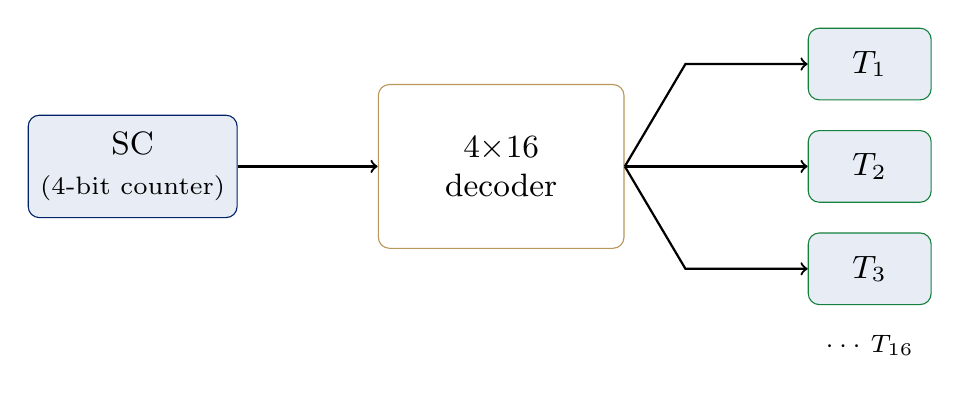
\begin{tikzpicture}[scale=1.30, transform shape,
        every node/.style={font=\small}]
      \node[draw=primary-blue, fill=light-bg, rounded corners,
            minimum width=2.0cm, minimum height=1.0cm, align=center] (SC) at (0,0) {SC \\ \scriptsize (4-bit counter)};
      \node[draw=primary-gold, fill=white, rounded corners,
            minimum width=2.4cm, minimum height=1.6cm, align=center] (DEC) at (3.6,0) {$4{\times}16$\\decoder};
      \draw[->, thick] (SC.east) -- (DEC.west);
      \node[draw=positive, fill=light-bg, rounded corners,
            minimum width=1.2cm, minimum height=0.7cm, align=center] (T1) at (7.2,1.0) {$T_1$};
      \node[draw=positive, fill=light-bg, rounded corners,
            minimum width=1.2cm, minimum height=0.7cm, align=center] (T2) at (7.2,0) {$T_2$};
      \node[draw=positive, fill=light-bg, rounded corners,
            minimum width=1.2cm, minimum height=0.7cm, align=center] (T3) at (7.2,-1.0) {$T_3$};
      \draw[->, thick] (DEC.east) -- (5.4,1.0) -- (T1.west);
      \draw[->, thick] (DEC.east) -- (5.4,0) -- (T2.west);
      \draw[->, thick] (DEC.east) -- (5.4,-1.0) -- (T3.west);
      \node[font=\scriptsize] at (7.2,-1.75) {$\cdots\,T_{16}$};
    \end{tikzpicture}
  \end{center}
  \footnotesize \cite{Mano1993_computer_system_architecture} --- cf.\ Fig.~5-6, p.137
  (the sequence-counter/timing-decoder portion of the control unit).
\end{frame}

\begin{frame}{How \texttt{SC} Advances}
  \begin{itemize}
    \item Every clock pulse, by default: $SC \gets [SC] + 1$ --- the counter just
      counts up, and the step decoder's one-hot output moves to the next $T_i$.
    \item At the \emph{last} step of an instruction, the control unit instead
      asserts $SC_{\text{clear}}$: $SC \gets 0$, which returns the decoder to $T_1$ ---
      signaling ``this instruction is done; begin fetching the next one.''
    \item Without $SC_{\text{clear}}$, the counter would keep counting forever with no
      instruction ever finishing.
  \end{itemize}
  \begin{exampleblock}{Applied to our trace}
    For \texttt{R1} $\gets$ \texttt{R2+R3}, $SC_{\text{clear}}$ fires at $T_3$ --- the last
    step of this instruction.
  \end{exampleblock}
\end{frame}

\begin{frame}{Worked Trace Revisited: Where \texttt{SC} Points}
  \footnotesize
  \begin{tabular}{@{}cccl@{}}
    \toprule
    \textbf{Step} & \textbf{SC value} & \textbf{Active line} & \textbf{RTL} \\
    \midrule
    $T_1$ & 0 & $T_1=1$ & $Y \gets [R2]$ \\
    $T_2$ & 1 & $T_2=1$ & $Z \gets [Y] + [R3]$ \\
    $T_3$ & 2 & $T_3=1$, $SC_{\text{clear}}=1$ & $R1 \gets [Z]$, then $SC \gets 0$ \\
    \bottomrule
  \end{tabular}
  \vspace{0.3cm}
  \key{This is the piece Week 5 was missing}: \texttt{SC} plus the step decoder
  \emph{is} the hardware that turns ``now it's $T_2$'' from something we wrote by
  hand into something the circuit does on its own, every cycle.
\end{frame}

\begin{frame}{Socratic Check: What Happens After $T_3$?}
  \begin{alertblock}{Question}
    Suppose we forgot to wire up $SC_{\text{clear}}$. What would the hardware do after
    $T_3$?
  \end{alertblock}
  \begin{itemize}
    \item \texttt{SC} would keep incrementing: $T_4, T_5, \dots$ forever.
    \item The step decoder would produce one-hot lines for steps that
      \emph{no instruction defines any signals for} --- the datapath would simply
      idle, and the next instruction would never be fetched.
    \item $SC_{\text{clear}}$ is not optional bookkeeping --- it is what makes the control
      unit cycle through instructions at all, rather than freezing after the first
      one.
  \end{itemize}
\end{frame}

\transitionslide{But different instructions need different micro-operations at each step --- how does hardware know which?}

% =============================================================================
% ACT 3 --- HARDWIRED CONTROL UNIT DESIGN
% =============================================================================
\section{Hardwired Control Unit Design}

\begin{frame}{The Missing Piece: Opcode Decoding}
  \begin{block}{Socratic question}
    \texttt{SC} tells the control unit \emph{when} (which $T_i$). But
    $Y_{\text{in}}$ should fire at $T_1$ for an \texttt{ADD}, while a \texttt{LOAD}
    instruction needs something completely different at its $T_1$. \texttt{SC}
    alone cannot know \emph{which} instruction is running.
  \end{block}
  \begin{itemize}
    \item New notation: $D_i$ --- a one-hot \key{opcode decoder} output, where
      $D_{\text{ADD}} = 1$ exactly when the \texttt{IR} holds the \texttt{ADD}
      opcode (and every other $D_j = 0$).
    \item Every control signal will turn out to depend on \emph{both} an opcode
      line ($D_i$) and a step line ($T_j$) --- never one alone.
  \end{itemize}
\end{frame}

\begin{frame}{Two Decoders Feed the Control Matrix}
  \begin{center}
    % Diagram: IR feeds an opcode decoder (D_i lines); SC feeds a step decoder
    % (T_j lines); the I flip-flop (bit 15, loaded from IR) feeds the matrix
    % directly; all three converge on the control matrix, which outputs the
    % control signals. Redrawn to match Mano Fig. 5-6 (p.137): a 3x8
    % operation decoder, a 4x16 timing decoder, and the I flip-flop are
    % three of the inputs to the control logic gates (IR bits 0-11 are the
    % fourth -- noted in prose below, omitted from the diagram for clarity).
    % This course numbers steps from T1 (Mano numbers from T0 -- see the
    % SC frame's note), so the timing decoder's outputs are T1..T16 here.
    % Coordinates: (x, y)
    %   IR box at (0, 1.8); "3x8 decoder" at (3.2, 1.8); D_i label at (6.0, 2.3)
    %   I flip-flop at (0, 0) -- bit 15, loaded via a short arrow from IR.south
    %     (0.4cm+ clear of IR's bottom edge y=1.4 and SC's top edge y=-1.4),
    %     feeds matrix directly at height 0; same primary-blue storage-element
    %     color as IR/SC (not the gate-neutral color, since it's a register)
    %   SC box at (0, -1.8); "4x16 decoder" at (3.2, -1.8); T_j label at (6.0, -2.3)
    %   Control matrix box at (9.6, 0), tall, receiving D_i/I/T_j as single
    %     unbroken paths (ODEC/IFF/SDEC -> elbow at x=8.0 -> MAT.west), one arrowhead each
    %   Control signals fan out right of matrix at (13.0, 0.9) and (13.0, -0.9)
    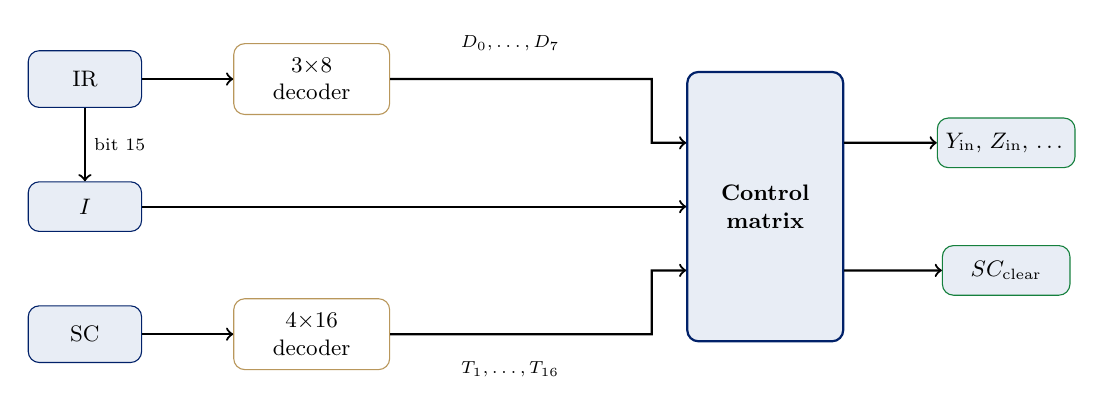
\begin{tikzpicture}[scale=0.90, transform shape,
        every node/.style={font=\small}]
      \node[draw=primary-blue, fill=light-bg, rounded corners,
            minimum width=1.6cm, minimum height=0.8cm, align=center] (IR) at (0,1.8) {IR};
      \node[draw=primary-gold, fill=white, rounded corners,
            minimum width=2.2cm, minimum height=1.0cm, align=center] (ODEC) at (3.2,1.8) {$3{\times}8$\\decoder};
      \draw[->, thick] (IR.east) -- (ODEC.west);
      \node[font=\scriptsize] at (6.0,2.3) {$D_0, \dots, D_7$};
      \node[draw=primary-blue, fill=light-bg, rounded corners,
            minimum width=1.6cm, minimum height=0.7cm, align=center] (IFF) at (0,0) {$I$};
      \draw[->, thick] (IR.south) -- node[midway, right, font=\scriptsize] {bit 15} (IFF.north);
      \node[draw=primary-blue, fill=light-bg, rounded corners,
            minimum width=1.6cm, minimum height=0.8cm, align=center] (SC) at (0,-1.8) {SC};
      \node[draw=primary-gold, fill=white, rounded corners,
            minimum width=2.2cm, minimum height=1.0cm, align=center] (SDEC) at (3.2,-1.8) {$4{\times}16$\\decoder};
      \draw[->, thick] (SC.east) -- (SDEC.west);
      \node[font=\scriptsize] at (6.0,-2.3) {$T_1, \dots, T_{16}$};
      \node[draw=primary-blue, thick, fill=light-bg, rounded corners,
            minimum width=2.2cm, minimum height=3.8cm, align=center]
            (MAT) at (9.6,0) {\textbf{Control}\\\textbf{matrix}};
      \draw[->, thick] (ODEC.east) -- (8.0,1.8) |- (MAT.west |- 0,0.9);
      \draw[->, thick] (IFF.east) -- (MAT.west |- 0,0);
      \draw[->, thick] (SDEC.east) -- (8.0,-1.8) |- (MAT.west |- 0,-0.9);
      \node[draw=positive, fill=light-bg, rounded corners,
            minimum width=1.8cm, minimum height=0.7cm, align=center] (OUT1) at (13.0,0.9) {$Y_{\text{in}}$, $Z_{\text{in}}$, \dots};
      \node[draw=positive, fill=light-bg, rounded corners,
            minimum width=1.8cm, minimum height=0.7cm, align=center] (OUT2) at (13.0,-0.9) {$SC_{\text{clear}}$};
      \draw[->, thick] (MAT.east |- 0,0.9) -- (OUT1.west);
      \draw[->, thick] (MAT.east |- 0,-0.9) -- (OUT2.west);
    \end{tikzpicture}
  \end{center}
  Every control signal is a Boolean function of the $D_i$ lines, the $T_j$
  lines, and (for indirect-addressing-sensitive signals) the $I$ flip-flop
  together --- \texttt{IR} bits 0--11 also feed the control logic gates
  directly (omitted above for clarity) --- cf.\ Mano, Fig.~5-6, p.137
  \cite{Mano1993_computer_system_architecture}.
\end{frame}

\begin{frame}{Building the State Table for \texttt{R1} $\gets$ \texttt{R2+R3}}
  \footnotesize
  \begin{tabular}{@{}cll@{}}
    \toprule
    \textbf{Step} & \textbf{RTL} & \textbf{Control signals active} \\
    \midrule
    $T_1$ & $Y \gets [R2]$            & $R2_{\text{out}}, Y_{\text{in}}$ \\
    $T_2$ & $Z \gets [Y] + [R3]$      & $R3_{\text{out}}$, ALU$=$add, $Z_{\text{in}}$ \\
    $T_3$ & $R1 \gets [Z]$            & $Z_{\text{out}}, R1_{\text{in}}, SC_{\text{clear}}$ \\
    \bottomrule
  \end{tabular}
  \vspace{0.3cm}
  \begin{exampleblock}{This is the state table}
    Every signal in the ``active'' column is only asserted when \emph{both}
    $D_{\text{ADD}} = 1$ \emph{and} the listed $T_i = 1$. The state table is the
    bridge between the RTL trace we already know and the Boolean equations we
    derive next.
  \end{exampleblock}
\end{frame}

\begin{frame}{From State Table to Boolean Equations}
  Reading straight off the state table for \texttt{ADD} (opcode line $D_{\text{ADD}}$):
  \begin{align*}
    Y_{\text{in}} &= D_{\text{ADD}} \cdot T_1 \\
    Z_{\text{in}} &= D_{\text{ADD}} \cdot T_2 \\
    R1_{\text{in}} &= D_{\text{ADD}} \cdot T_3 \\
    SC_{\text{clear}} &= D_{\text{ADD}} \cdot T_3
  \end{align*}
  \begin{itemize}
    \item Each equation is just: ``this signal fires when this instruction is
      running \emph{and} we are at this step.''
    \item If a \emph{different} instruction also needs $Z_{\text{in}}$ at some step, its
      term gets \textbf{OR}'d into the same equation --- covered next.
  \end{itemize}
\end{frame}

\begin{frame}{Worked Example: Deriving $Z_{\text{in}}$ by Hand}
  \begin{block}{Suppose \texttt{SUB} also uses $Z$ to hold its result, at its own $T_2$}
    \texttt{SUB} has an identical 3-step shape to \texttt{ADD}, differing only in
    the ALU function selected at $T_2$.
  \end{block}
  \begin{enumerate}
    \item From the \texttt{ADD} state table: $Z_{\text{in}}$ fires at $D_{\text{ADD}} \cdot T_2$.
    \item From the \texttt{SUB} state table: $Z_{\text{in}}$ also fires at $D_{\text{SUB}} \cdot T_2$.
    \item \textbf{Any} instruction whose state table lists $Z_{\text{in}}$ at $T_2$
      contributes an OR term.
  \end{enumerate}
  \[
    Z_{\text{in}} = (D_{\text{ADD}} \cdot T_2) + (D_{\text{SUB}} \cdot T_2) = T_2 \cdot (D_{\text{ADD}} + D_{\text{SUB}})
  \]
  \key{This is the general pattern}: every control signal is an OR, across all
  instructions that use it, of (opcode line $\cdot$ step line).
\end{frame}

\begin{frame}{The Control Matrix as Actual Logic Gates}
  \begin{center}
    % Diagram: AND-OR realization of Z_in = (D_ADD . T2) + (D_SUB . T2).
    % Colors follow the deck convention: neutral/white = logic gate (AND, OR
    % are the same class of object, so they share one style); positive = the
    % control-signal output.
    % Coordinates: (x, y)
    %   D_ADD label at (-0.75, 1.9), T2 label at (-0.75, 1.1) -> AND gate 1 at (3.0, 1.5),
    %     height 1.4 so wires enter the straight west edge (y=0.8..2.2), not the corner
    %   D_SUB label at (-0.75, -1.1), T2 label at (-0.75, -1.9) -> AND gate 2 at (3.0, -1.5)
    %   OR gate at (6.2, 0), west edge x=5.7 -- both AND outputs route via x=5.3
    %     (0.4 clear of the OR box) then straight into OR.west, no backtracking
    %   Z_in output at (9.0, 0)
    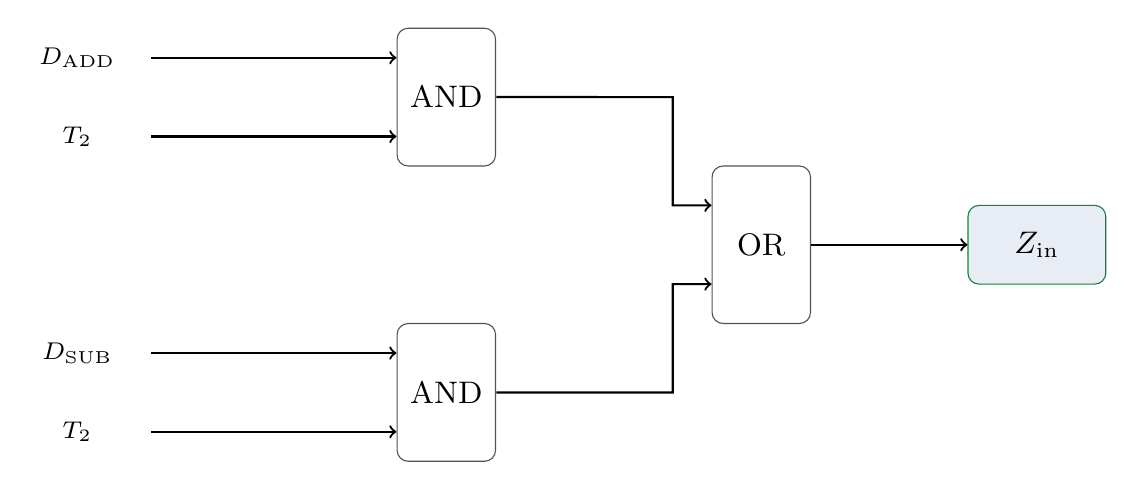
\begin{tikzpicture}[scale=1.25, transform shape,
        every node/.style={font=\small}]
      \node[font=\scriptsize] at (-0.75,1.9) {$D_{\text{ADD}}$};
      \node[font=\scriptsize] at (-0.75,1.1) {$T_2$};
      \node[draw=neutral, fill=white, rounded corners,
            minimum width=1.0cm, minimum height=1.4cm, align=center] (AND1) at (3.0,1.5) {AND};
      \draw[->, thick] (0,1.9) -- (AND1.west |- 0,1.9);
      \draw[->, thick] (0,1.1) -- (AND1.west |- 0,1.1);
      \node[font=\scriptsize] at (-0.75,-1.1) {$D_{\text{SUB}}$};
      \node[font=\scriptsize] at (-0.75,-1.9) {$T_2$};
      \node[draw=neutral, fill=white, rounded corners,
            minimum width=1.0cm, minimum height=1.4cm, align=center] (AND2) at (3.0,-1.5) {AND};
      \draw[->, thick] (0,-1.1) -- (AND2.west |- 0,-1.1);
      \draw[->, thick] (0,-1.9) -- (AND2.west |- 0,-1.9);
      \node[draw=neutral, fill=white, rounded corners,
            minimum width=1.0cm, minimum height=1.6cm, align=center] (OR) at (6.2,0) {OR};
      \draw[->, thick] (AND1.east) -- (5.3,1.5) -- (5.3,0.4) -- (OR.west |- 0,0.4);
      \draw[->, thick] (AND2.east) -- (5.3,-1.5) -- (5.3,-0.4) -- (OR.west |- 0,-0.4);
      \node[draw=positive, fill=light-bg, rounded corners,
            minimum width=1.4cm, minimum height=0.8cm, align=center] (OUT) at (9.0,0) {$Z_{\text{in}}$};
      \draw[->, thick] (OR.east) -- (OUT.west);
    \end{tikzpicture}
  \end{center}
  \muted{Two AND gates (one per instruction that needs $Z_{\text{in}}$ at $T_2$), one OR
  gate combining them --- this is literally what ``hardwired'' means.}
\end{frame}

\begin{frame}{Full Hardwired Control Unit Block Diagram}
  \begin{center}
    % Diagram: capstone assembly -- IR and SC/clock both feed decoders, flags
    % feed in separately, everything converges on the control matrix, which
    % drives the datapath (register gating, ALU select, memory R/W) and also
    % feeds back to clear/advance SC. Redrawn to match Mano Fig. 5-6 (p.137)
    % at its core (3x8 operation decoder + 4x16 timing decoder + control
    % logic gates); Flags/Clock as separate explicit inputs and the SC
    % feedback loop are this course's pedagogical extension of that core,
    % drawn out for clarity (the book folds clock timing into the SC/decoder
    % relationship itself rather than showing it as a fourth input box).
    % Coordinates: (x, y)
    %   IR at (0, 2.2); Flags at (0, 0.7); Clock at (0, -0.8); (feed control matrix)
    %   SC at (0, -2.3) -> step decoder at (3.0,-2.3) -> matrix
    %   Opcode decoder at (3.0, 2.2) between IR and matrix
    %   Control matrix (large box) at (6.4, 0)
    %   Datapath outputs at (10.2, 1.2) and (10.2, -0.2)
    %   Feedback SC_clear/advance from matrix back down to SC at (10.2,-1.6) -> loops left to SC
    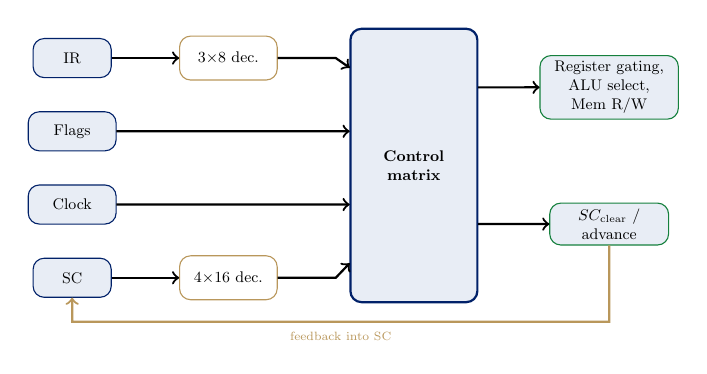
\begin{tikzpicture}[scale=0.62, transform shape,
        every node/.style={font=\small}]
      \node[draw=primary-blue, fill=light-bg, rounded corners,
            minimum width=1.6cm, minimum height=0.8cm, align=center] (IR) at (0,2.2) {IR};
      \node[draw=primary-gold, fill=white, rounded corners,
            minimum width=2.0cm, minimum height=0.9cm, align=center] (ODEC) at (3.2,2.2) {$3{\times}8$ dec.};
      \draw[->, thick] (IR.east) -- (ODEC.west);
      \node[draw=primary-blue, fill=light-bg, rounded corners,
            minimum width=1.8cm, minimum height=0.8cm, align=center] (FLAGS) at (0,0.7) {Flags};
      \node[draw=primary-blue, fill=light-bg, rounded corners,
            minimum width=1.8cm, minimum height=0.8cm, align=center] (CLK) at (0,-0.8) {Clock};
      \node[draw=primary-blue, fill=light-bg, rounded corners,
            minimum width=1.6cm, minimum height=0.8cm, align=center] (SC) at (0,-2.3) {SC};
      \node[draw=primary-gold, fill=white, rounded corners,
            minimum width=2.0cm, minimum height=0.9cm, align=center] (SDEC) at (3.2,-2.3) {$4{\times}16$ dec.};
      \draw[->, thick] (SC.east) -- (SDEC.west);
      \node[draw=primary-blue, thick, fill=light-bg, rounded corners,
            minimum width=2.6cm, minimum height=5.6cm, align=center]
            (MAT) at (7.0,0) {\textbf{Control}\\\textbf{matrix}};
      \draw[->, thick] (ODEC.east) -- (5.4,2.2) -- (MAT.west |- 0,2.0);
      \draw[->, thick] (FLAGS.east) -- (5.4,0.7) -- (MAT.west |- 0,0.7);
      \draw[->, thick] (CLK.east) -- (5.4,-0.8) -- (MAT.west |- 0,-0.8);
      \draw[->, thick] (SDEC.east) -- (5.4,-2.3) -- (MAT.west |- 0,-2.0);
      \node[draw=positive, fill=light-bg, rounded corners, text width=2.6cm,
            minimum height=0.8cm, align=center] (OUT1) at (11.0,1.6) {Register gating, ALU select, Mem R/W};
      \draw[->, thick] (MAT.east |- 0,1.6) -- (OUT1.west);
      \node[draw=positive, fill=light-bg, rounded corners, text width=2.2cm,
            minimum height=0.8cm, align=center] (OUT2) at (11.0,-1.2) {$SC_{\text{clear}}$ / advance};
      \draw[->, thick] (MAT.east |- 0,-1.2) -- (OUT2.west);
      \draw[->, thick, primary-gold] (OUT2.south) -- (11.0,-3.2) -- (0,-3.2) -- (SC.south);
      \node[font=\scriptsize, primary-gold] at (5.5,-3.5) {feedback into SC};
    \end{tikzpicture}
  \end{center}
  \footnotesize cf.\ Mano, Fig.~5-6, p.137 (core: two decoders + SC + control
  logic gates), extended with explicit Flags/Clock inputs and the SC
  feedback loop \cite{Mano1993_computer_system_architecture,Hamacher2002_computer_organization}.
\end{frame}

\begin{frame}{Socratic Check: Adding a New Instruction}
  \begin{alertblock}{Question}
    Suppose we now add a \texttt{MUL} instruction that also uses $Z$ at its own
    $T_2$. What has to change in the hardwired control unit we just built?
  \end{alertblock}
  \begin{itemize}
    \item The opcode decoder needs a \emph{new output line}, $D_{\text{MUL}}$.
    \item Every equation for a signal \texttt{MUL} needs (e.g.\ $Z_{\text{in}}$) must be
      \textbf{re-derived}, and a new AND gate ($D_{\text{MUL}} \cdot T_2$) must be
      physically wired into the existing OR gate.
    \item This is not a software change --- it is new gates, on the actual chip,
      for \emph{every} signal the new instruction touches.
  \end{itemize}
\end{frame}

\transitionslide{Fast, but rigid --- what does that cost us?}

% =============================================================================
% ACT 4 --- TRADE-OFFS AND SYNTHESIS
% =============================================================================
\section{Trade-offs and Synthesis}

\begin{frame}{Hardwired Control: Trade-offs}
  \begin{block}{Cost vs.\ flexibility}
    \begin{itemize}
      \item \good{Pro}: pure combinational logic --- control signals appear the
        \emph{same cycle}, with no extra memory-access delay.
      \item \good{Pro}: no wasted circuitry --- the gates that exist are exactly
        the ones the ISA needs, nothing more.
      \item \bad{Con}: adding, removing, or fixing a bug in one instruction means
        re-deriving equations and \emph{physically rewiring} logic gates.
      \item \bad{Con}: the control matrix grows with the number of instructions
        $\times$ the number of signals --- verifying it by hand gets harder fast.
    \end{itemize}
  \end{block}
\end{frame}

\begin{frame}{Where This Breaks Down}
  \begin{itemize}
    \item Our worked example had \emph{one} instruction (\texttt{ADD}), 3 steps,
      and a handful of signals --- the equations fit on one slide.
    \item A real ISA has dozens to hundreds of instructions, each with its own
      state table, each contributing AND terms to \emph{every} shared signal's OR
      equation.
    \item Every new instruction, every microarchitectural bug fix, means
      re-deriving Boolean equations and re-wiring gates by hand --- design and
      verification cost explodes with ISA complexity \cite{Stallings2015_computer_organization}.
  \end{itemize}
\end{frame}

\begin{frame}{Bridge to Week 7}
  \begin{exampleblock}{A different idea}
    What if, instead of wiring $Y_{\text{in}}, Z_{\text{in}}, R1_{\text{in}}, \dots$ directly
    into logic gates, we simply \emph{wrote them down} --- one row per control
    step, stored in a small memory --- and let a counter step through the rows?
  \end{exampleblock}
  \begin{itemize}
    \item Adding a new instruction becomes: write new rows into memory, not
      redesign gates.
    \item The trade-off flips: slightly slower per step (a memory read), far
      easier to design, verify, and modify.
    \item That is \key{microprogrammed control} --- next week, we rebuild
      \emph{this same} \texttt{R1} $\gets$ \texttt{R2+R3} control unit that way.
  \end{itemize}
\end{frame}

\begin{frame}{The Two Threads Meet}
  \begin{block}{Control-step count depends on the bus organization (Week 5)}
    \begin{itemize}
      \item Single-bus: 3 states ($T_1, T_2, T_3$) $\Rightarrow$ \texttt{SC} needs 2
        bits, step decoder has 3 outputs, and \texttt{ADD}'s state table has 3 rows.
      \item Three-bus: 1 state ($T_1$ only) $\Rightarrow$ \texttt{SC} barely needs
        to exist, and \texttt{ADD}'s state table has 1 row.
    \end{itemize}
  \end{block}
  \begin{itemize}
    \item Fewer control steps means a \emph{smaller} state table and fewer AND/OR
      gates in the control matrix --- the cost moves from control logic into bus
      wiring instead.
    \item Neither the datapath choice (Week 5) nor the control unit choice
      (Week 6) is free --- every design decision moves cost somewhere else on the
      chip.
  \end{itemize}
\end{frame}

\begin{frame}{Summary}
  \begin{itemize}
    \item \key{Control unit} $=$ the hardware that reads (opcode, step, flags)
      and asserts control signals for every other component, every cycle.
    \item \key{Sequence counter (\texttt{SC})} $+$ step decoder generate
      $T_1, T_2, \dots$ automatically; $SC_{\text{clear}}$ resets to $T_1$ at an
      instruction's last step.
    \item \key{Opcode decoder} produces one-hot $D_i$ lines; every control signal
      is an OR, across instructions, of $(D_i \cdot T_j)$ terms --- the
      \textbf{state table} makes this systematic.
    \item \key{Hardwired control}: state table $\to$ Boolean equations $\to$
      AND/OR gates. Fast, but rigid --- new instructions mean new gates, wired by
      hand.
    \item This rigidity is exactly what motivates \key{microprogrammed control}
      (Week 7): store control words in memory instead of wiring them into gates.
  \end{itemize}
\end{frame}

\begin{frame}{References}
  \footnotesize
  \bibliographystyle{plain}
  \bibliography{../../Bibliography_base}
\end{frame}

\end{document}
